% Gabarit pandoc des corrigés publiés (brut et guidé). Contenu sans marque ni nom de site.
% Compilation : lualatex (latexmk -lualatex).
% Le Markdown reste la source unique : ne pas éditer ce fichier .tex à la main.
\documentclass[11pt,a4paper]{article}

% --- Moteur, polices (Latin Modern) et langue ---------------------------------
\usepackage{iftex}
\ifLuaTeX\else\errmessage{Ce document se compile avec lualatex}\fi
\usepackage{amsmath,amssymb,mathtools}
\usepackage{fontspec}
% mathrm=sym : \mathrm prend ses glyphes dans la police mathématique (ℓ, μ, Ω), comme KaTeX.
\usepackage[math-style=TeX,bold-style=TeX,mathrm=sym]{unicode-math}
% Repli pour les glyphes absents de Latin Modern (indices et exposants Unicode,
% flèches, filets des schémas en texte, symboles) : DejaVu, puis Latin Modern Math
% (ℓ, lettres mathématiques Unicode des légendes).
\directlua{
  luaotfload.add_fallback("repliTexte", {"DejaVuSerif:mode=harf;", "DejaVuSans:mode=harf;", "file:latinmodern-math.otf:mode=harf;"})
  luaotfload.add_fallback("repliMono", {"DejaVuSansMono:mode=harf;", "DejaVuSans:mode=harf;", "file:latinmodern-math.otf:mode=harf;"})
}
\setmainfont{Latin Modern Roman}[RawFeature={fallback=repliTexte}]
\setsansfont{Latin Modern Sans}[RawFeature={fallback=repliTexte}]
\setmonofont{Latin Modern Mono}[RawFeature={fallback=repliMono}]
\setmathfont{Latin Modern Math}
\usepackage[french]{babel}
\frenchsetup{SmallCapsFigTabCaptions=false}

% --- Mise en page --------------------------------------------------------------
\usepackage[a4paper,margin=2.2cm,headheight=14pt,footskip=1.2cm]{geometry}
\usepackage{microtype}
\setlength{\emergencystretch}{4em}
\tolerance=1500
\setlength{\parindent}{0pt}
\setlength{\parskip}{0.55\baselineskip plus 2pt minus 1pt}
\usepackage{xcolor}
% Gris nommés : babel-french rend « ! » actif dans le document.
\definecolor{gris2}{gray}{0.98}
\definecolor{gris3}{gray}{0.97}
\definecolor{gris5}{gray}{0.95}
\definecolor{gris35}{gray}{0.65}
\definecolor{gris40}{gray}{0.60}
\definecolor{gris45}{gray}{0.55}
\definecolor{gris50}{gray}{0.50}
\definecolor{gris55}{gray}{0.45}
\definecolor{gris60}{gray}{0.40}
\definecolor{gris65}{gray}{0.35}
\definecolor{gris70}{gray}{0.30}
\definecolor{gris80}{gray}{0.20}
\definecolor{gris85}{gray}{0.15}
\usepackage{graphicx}
\usepackage{float}
\usepackage{caption}
\captionsetup{font=small,labelformat=empty,justification=centering}
\usepackage{booktabs,longtable,array,multirow,calc}
\usepackage{siunitx}
\sisetup{locale=FR}
\usepackage[version=4]{mhchem}
\usepackage{listings}
\usepackage{fancyhdr}
\usepackage{lastpage}
\usepackage[most]{tcolorbox}
\usepackage{enumitem}
\setlist{nosep,leftmargin=*,topsep=2pt}
\usepackage[hidelinks,unicode]{hyperref}
\usepackage{bookmark}
\hypersetup{pdftitle={Centrale-Supélec PSI — Physique-chimie 2 2026},pdfauthor={Rédigé par IA},pdfcreator={LaTeX},pdfsubject={Corrigé guidé}}
\usepackage{xurl}

% --- Pandoc : listes, tableaux, figures ----------------------------------------
\providecommand{\passthrough}[1]{#1}
\providecommand{\tightlist}{\setlength{\itemsep}{0pt}\setlength{\parskip}{0pt}}

\makeatletter
\def\maxwidth{\ifdim\Gin@nat@width>\linewidth\linewidth\else\Gin@nat@width\fi}
\def\maxheight{\ifdim\Gin@nat@height>0.55\textheight 0.55\textheight\else\Gin@nat@height\fi}
\makeatother
\setkeys{Gin}{width=\maxwidth,height=\maxheight,keepaspectratio}
\setcounter{secnumdepth}{-\maxdimen}
\providecommand{\pandocbounded}[1]{#1}
\usepackage{longtable,booktabs,array}

% --- Code (listings) -----------------------------------------------------------
\lstset{
  basicstyle=\ttfamily\small,
  columns=fullflexible,
  keepspaces=true,
  breaklines=true,
  breakatwhitespace=false,
  postbreak=\mbox{\textcolor{gris50}{$\hookrightarrow$}\space},
  frame=single,
  rulecolor=\color{gris35},
  framesep=4pt,
  xleftmargin=5pt,xrightmargin=5pt,
  backgroundcolor=\color{gris3},
  keywordstyle=\bfseries,
  commentstyle=\color{gris65},
  stringstyle=\color{gris80},
  showstringspaces=false,
  tabsize=4,
  extendedchars=true,
  aboveskip=6pt,belowskip=6pt,
}

% --- Macros des corrigés (KaTeX ↔ LaTeX) ---------------------------------------
% Les corrigés sont écrits pour KaTeX : on définit ici ce que KaTeX connaît et
% que LaTeX n'a pas, sans jamais retoucher le Markdown.
\providecommand{\R}{\mathbb{R}}
\providecommand{\N}{\mathbb{N}}
\providecommand{\Z}{\mathbb{Z}}
\providecommand{\Q}{\mathbb{Q}}
\providecommand{\C}{\mathbb{C}}
\providecommand{\dd}{\mathrm{d}}
\providecommand{\llbracket}{\lBrack}
\providecommand{\rrbracket}{\rBrack}
\providecommand{\lBrace}{\lbrace}
\providecommand{\rBrace}{\rbrace}
\providecommand{\Box}{\square}
\providecommand{\Diamond}{\lozenge}
\providecommand{\varnothing}{\emptyset}
\providecommand{\argmax}{\operatorname*{arg\,max}}
\providecommand{\argmin}{\operatorname*{arg\,min}}
\renewcommand{\leq}{\leqslant}
\renewcommand{\geq}{\geqslant}

% Équation hors texte : réduite à la largeur de la ligne si elle déborde.
\newsavebox{\boiteequation}
\newcommand{\equationajustee}[1]{%
  \sbox{\boiteequation}{$\displaystyle #1$}%
  \ifdim\wd\boiteequation>\linewidth
    \[\resizebox{\linewidth}{!}{\usebox{\boiteequation}}\]%
  \else
    \[#1\]%
  \fi}

% --- Encadrés pédagogiques (sobres, lisibles en noir et blanc) -----------------
\tcbset{
  encadre/.style={
    enhanced,breakable,sharp corners,
    colback=white,colframe=gris55,
    boxrule=0.4pt,leftrule=2.2pt,
    left=6pt,right=6pt,top=3pt,bottom=3pt,
    before skip=6pt,after skip=6pt,
    fonttitle=\bfseries\small,coltitle=black,
    attach title to upper,after title={\quad},
    parbox=false,
  }
}
\newtcolorbox{indication}[1]{encadre,colframe=gris45,colback=gris2,title={Indication~#1}}
\newtcolorbox{methode}{encadre,colframe=gris70,title={Méthode}}
\newtcolorbox{piege}{encadre,colframe=gris85,boxrule=0.8pt,leftrule=2.2pt,title={Piège}}
\newtcolorbox{jury}{encadre,colframe=gris60,colback=gris5,title={Jury}}
\newtcolorbox{encadrenote}{encadre,colframe=gris40}

% --- Titres de section ---------------------------------------------------------
\usepackage{titlesec}
\titleformat{\section}{\Large\bfseries}{}{0pt}{}
\titleformat{\subsection}{\large\bfseries}{}{0pt}{}
\titleformat{\subsubsection}{\normalsize\bfseries}{}{0pt}{}
\titlespacing*{\section}{0pt}{14pt plus 4pt minus 2pt}{6pt}
\titlespacing*{\subsection}{0pt}{10pt plus 3pt minus 2pt}{4pt}
\titlespacing*{\subsubsection}{0pt}{8pt plus 2pt minus 2pt}{2pt}

% --- En-tête et pied de page ---------------------------------------------------
\pagestyle{fancy}
\fancyhf{}
\fancyhead[L]{\small\textsc{Corrigé guidé} · Centrale-Supélec PSI}
\fancyhead[R]{\small Physique-chimie 2 2026}
\fancyfoot[L]{\footnotesize Corrigé rédigé par IA, non officiel}
\fancyfoot[R]{\footnotesize \thepage\,/\,\pageref*{LastPage}}
\renewcommand{\headrulewidth}{0.4pt}
\renewcommand{\footrulewidth}{0pt}
\fancypagestyle{plain}{\fancyhf{}\fancyfoot[R]{\footnotesize \thepage\,/\,\pageref*{LastPage}}\fancyfoot[L]{\footnotesize Corrigé rédigé par IA, non officiel}\renewcommand{\headrulewidth}{0pt}}

\begin{document}
\thispagestyle{plain}
\begin{center}
  {\small\scshape Corrigé guidé}\par\smallskip
  {\LARGE\bfseries Centrale-Supélec PSI — Physique-chimie 2 2026\par}\medskip
  {\large Centrale-Supélec · PSI · Physique-chimie 2 · 2026\par}
\end{center}
\vspace{2pt}\hrule\vspace{8pt}

\emph{Corrigé rédigé par IA, non officiel. Signalez toute erreur.}

\hypertarget{pruxe9sentation-du-sujet}{%
\section{Présentation du sujet}\label{pruxe9sentation-du-sujet}}

\textbf{Thème.} « Création d'un synthétiseur analogique rudimentaire ». Le sujet suit la chaîne d'un synthétiseur de type Minimoog, du clavier à l'oscillateur, puis aborde son refroidissement et la protection chimique de ses circuits imprimés. Durée 4 heures, calculatrice autorisée, \textbf{45 questions} en trois parties indépendantes de longueurs comparables.

\begin{longtable}[]{@{}
  >{\raggedright\arraybackslash}p{(\columnwidth - 4\tabcolsep) * \real{0.1573}}
  >{\raggedright\arraybackslash}p{(\columnwidth - 4\tabcolsep) * \real{0.3737}}
  >{\raggedright\arraybackslash}p{(\columnwidth - 4\tabcolsep) * \real{0.4390}}@{}}
\toprule\noalign{}
\begin{minipage}[b]{\linewidth}\raggedright
Partie
\end{minipage} & \begin{minipage}[b]{\linewidth}\raggedright
Contenu
\end{minipage} & \begin{minipage}[b]{\linewidth}\raggedright
Notions du programme
\end{minipage} \\
\midrule\noalign{}
\endhead
\bottomrule\noalign{}
\endlastfoot
A.I.1 (Q1--Q3) & Convertisseur linéaire/exponentiel à transistor & Lecture d'un modèle exponentiel, diviseur de tension \\
A.I.2 (Q4--Q8) & Dérive thermique, montage à deux transistors, compensation par thermistance CTP & Différentielle logarithmique, développement au premier ordre, choix argumenté \\
A.I.3 (Q9--Q12) & Transposeur d'octave à deux ALI & ALI idéal en régime linéaire, suiveur, sommateur, pont diviseur \\
A.II (Q13--Q20) & Oscillateur commandé en tension : intégrateur et comparateur à hystérésis & Régime saturé, oscillateur de relaxation, vitesse de balayage \\
B (Q21--Q32) & Ailette de refroidissement en aluminium & Loi de Fourier, loi de Newton, bilan sur une tranche, conditions aux limites, rendement d'ailette \\
C.I (Q33--Q39) & Nitruration du silicium & Grandeurs standard de réaction, \(K^\circ\), température de fin de réaction adiabatique, ordre 0, loi d'Arrhenius \\
C.II (Q40--Q45) & Croissance d'une couche de \(\mathrm{SiO_2}\) (modèle de Deal-Grove) & Oxydoréduction, flux molaires, résistances en série, régimes asymptotiques, quasi-stationnarité \\
\end{longtable}

\textbf{Question à prise d'initiative.} Seule la \textbf{Q8} a un numéro souligné : il faut proposer une modification du circuit, choisir un composant dans une table et chiffrer le gain obtenu. Le barème valorise une démarche explicitée.

\textbf{Difficulté et longueur.} Le sujet est long mais guidé, et les calculs restent courts. Ce qui départage les candidats, c'est la qualité des justifications (régime des ALI, choix des conditions aux limites, critère « quantitatif ») et la \textbf{confrontation des résultats numériques aux données} : seuil de \(0{,}0035\) en partie A, valeur de \(m\ell\) en partie B, températures de fusion en partie C. Trois questions demandent un graphe (Q15, Q19, Q44) et deux une lecture de courbe (Q31, Q39).

Deux coquilles de l'énoncé sont à repérer : \(\rho_{\mathrm{SiO_2}}\) vaut \(2{,}20\ \mathrm{g\cdot cm^{-3}}\) (et non \(\mathrm{kg\cdot m^{-3}}\)), et la « figure 13 » est la figure 12. La constante \(R\) n'est pas donnée : on la calcule par \(R=k_BN_A=8{,}31\ \mathrm{J\cdot K^{-1}\cdot mol^{-1}}\).

\textbf{Questions abordables à ne pas laisser passer.} Q2, Q5, Q9, Q10, Q11, Q12, Q13, Q15, Q18, Q21, Q23, Q24, Q25, Q26, Q30, Q33, Q35, Q38, Q40, Q41, Q42.

\textbf{Gestion du temps.} Comptez environ 1 h 40 pour la partie A (dont 20 min pour la Q8), 1 h pour la partie B, 1 h pour la partie C, et 20 min de relecture. Si la Q8 résiste, passez à la sous-partie I.3, qui en est indépendante.

\hypertarget{partie-a-cruxe9ation-dun-synthuxe9tiseur-analogique}{%
\section{Partie A --- Création d'un synthétiseur analogique}\label{partie-a-cruxe9ation-dun-synthuxe9tiseur-analogique}}

On part de la tension délivrée par une touche de clavier. On la rend exponentielle pour respecter la gamme (I.1), on la stabilise en température (I.2) et on la transpose d'octave (I.3). On construit ensuite l'oscillateur dont la fréquence est proportionnelle à cette tension (II). Les outils sont ceux de l'électronique de première année et de PSI : diviseur de tension, ALI idéal en régime linéaire ou saturé, intégrateur, comparateur à hystérésis.

\hypertarget{question-1}{%
\subsection{Question 1}\label{question-1}}

\begin{indication}{1}

Comparez deux lois : comment la tension du clavier dépend-elle du numéro d'octave, et comment la fréquence en dépend-elle ? L'une est arithmétique, l'autre géométrique.

\end{indication}

\begin{indication}{2}

Écrivez \(f({\mathrm{La}}_n)\) en fonction de \(f({\mathrm{La}}_0)\) et de \(n\). Exprimez \(n\) en fonction de \(V_{\mathrm{in},0}\), puis utilisez \(f\propto V_{\mathrm{in},1}\). Une puissance de 2 s'écrit comme une exponentielle.

\end{indication}

\hypertarget{solution}{%
\subsubsection{Solution}\label{solution}}

Le clavier délivre \(V_{\mathrm{in},0}=-5+n\) (en volts) pour le La\(_n\) : la tension est \textbf{affine} en l'octave. La fréquence, elle, est \textbf{géométrique} : \(f({\mathrm{La}}_n)=f({\mathrm{La}}_0)\,2^n\).

L'OCT donne \(f=\kappa V_{\mathrm{in},1}\). Sans bloc intermédiaire, \(f\) serait affine en \(V_{\mathrm{in},0}\) : les octaves seraient espacées d'un même écart de fréquence au lieu d'un même rapport, et la gamme serait fausse. Il faut un bloc qui transforme une progression arithmétique en progression géométrique, c'est-à-dire une exponentielle.

Avec \(n=V_{\mathrm{in},0}+5\) :

\equationajustee{\begin{aligned}
\kappa V_{\mathrm{in},1}&=f({\mathrm{La}}_0)\,2^{V_{\mathrm{in},0}+5}\\
&=32\,f({\mathrm{La}}_0)\,{\mathrm{e}}^{V_{\mathrm{in},0}\ln 2}
\end{aligned}}

On obtient la forme demandée, avec \(V_{\mathrm{ref}}=32f({\mathrm{La}}_0)/\kappa\) et

\equationajustee{\boxed{\alpha=\ln2\simeq0{,}693\ \mathrm{V^{-1}}}}

\begin{piege}

\(\alpha\) a une unité : l'argument d'une exponentielle est sans dimension, donc \(\alpha\) s'exprime en \(\mathrm{V^{-1}}\). Écrire « \(\alpha=0{,}693\) » tout court est une faute d'homogénéité.

\end{piege}

\hypertarget{question-2}{%
\subsection{Question 2}\label{question-2}}

\begin{indication}{1}

Si \(f\propto V_{\mathrm{in},1}\propto I_C\), que devient \(I_C\) quand on monte d'une octave ?

\end{indication}

\begin{indication}{2}

Formez le rapport de deux expressions d'Ebers-Moll à la même température : un facteur disparaît.

\end{indication}

\hypertarget{solution-1}{%
\subsubsection{Solution}\label{solution-1}}

Monter d'une octave double \(f\), donc \(I_C\). À température fixée, \(I_S(T)\) se simplifie :

\equationajustee{\begin{aligned}
2&=\frac{I_S\exp\big((V_{BE}+\Delta V_{BE})/v\big)}{I_S\exp\big(V_{BE}/v\big)}\\
&=\exp\Big(\frac{\Delta V_{BE}}{v(T)}\Big)
\end{aligned}}

d'où

\equationajustee{\boxed{\Delta V_{BE}=v(T)\ln2}}

À \(T=293{,}15\ \mathrm{K}\) :

\equationajustee{\begin{aligned}
v&=\frac{1{,}38\times10^{-23}\times293{,}15}{1{,}60\times10^{-19}}\\
&=25{,}3\ \mathrm{mV}
\end{aligned}}

donc \(\boxed{\Delta V_{BE}=17{,}5\ \mathrm{mV}}\).

\begin{methode}

Pour une loi exponentielle, un \textbf{rapport} constant de la grandeur de sortie correspond à un \textbf{écart} constant de l'argument. C'est la propriété qui permet à un clavier à « 1 V par octave » de fonctionner quelle que soit la note de départ.

\end{methode}

\begin{piege}

La température doit être en kelvins dans \(v=k_BT/q\). Avec \(T=20\), on trouverait une valeur environ quinze fois trop petite. Retenez l'ordre de grandeur \(v\approx25\ \mathrm{mV}\) à température ambiante.

\end{piege}

\hypertarget{question-3}{%
\subsection{Question 3}\label{question-3}}

\begin{indication}{1}

Que dire du courant dans \(R\) et dans \(R'\) si \(I_B=0\) ? Quel théorème donne alors \(V_{BE}\) ?

\end{indication}

\begin{indication}{2}

Reportez \(V_{BE}\) dans Ebers-Moll et identifiez le coefficient de \(V_{\mathrm{in},0}\) dans l'exponentielle. « En considérant 20 °C » appelle une application numérique, à comparer à Q1.

\end{indication}

\hypertarget{solution-2}{%
\subsubsection{Solution}\label{solution-2}}

Comme \(I_B=0\), \(R\) et \(R'\) sont en série, parcourues par le même courant. Le diviseur de tension donne

\equationajustee{V_{BE}=\frac{R'}{R+R'}V_{\mathrm{in},0}}

L'émetteur est à la masse et \(V_{\mathrm{in},1}=\mu I_C\) (\(\mu\) constante), donc

\equationajustee{V_{\mathrm{in},1}=\mu I_S(T)\exp\Big(\frac{R'}{(R+R')\,v(T)}V_{\mathrm{in},0}\Big)}

On identifie :

\equationajustee{\boxed{V_{\mathrm{ref}}=\mu I_S(T)}}

\equationajustee{\boxed{\alpha=\frac{R'}{(R+R')\,v(T)}}}

C'est bien la forme \(g(V_{\mathrm{in},0})\). À \(20\ ^\circ\mathrm{C}\), on a \(R'/(R+R')=1{,}00/57{,}0=1{,}754\times10^{-2}\), d'où

\equationajustee{\begin{aligned}
\alpha&=\frac{1{,}754\times10^{-2}}{2{,}528\times10^{-2}}\\
&=0{,}694\ \mathrm{V^{-1}}
\end{aligned}}

soit un écart de \(0{,}1\ \%\) à \(\ln2\).

\textbf{Le couple \((R,R')\) réalise le convertisseur voulu} : une variation d'un volt de \(V_{\mathrm{in},0}\) produit \(\Delta V_{BE}=17{,}5\ \mathrm{mV}\), l'écart exigé en Q2.

\begin{jury}

Pour un « montrer que », deux étapes sont attendues : établir la forme (ici le diviseur de tension), puis vérifier la valeur numérique demandée. S'arrêter à la forme laisse la moitié de la question sans réponse.

\end{jury}

\hypertarget{question-4}{%
\subsection{Question 4}\label{question-4}}

\begin{indication}{1}

Commencez par trouver la tension \(V_{\mathrm{in},0}\), puis \(V_{BE}\), associées au La\(_3\). Cette tension dépend-elle de la température ?

\end{indication}

\begin{indication}{2}

\(I_C\) est le produit de deux facteurs qui dépendent de \(T\). Faites varier l'un en gelant l'autre, puis comparez chaque effet au seuil de \(0{,}0035\).

\end{indication}

\hypertarget{solution-3}{%
\subsubsection{Solution}\label{solution-3}}

Le La\(_3\) est trois octaves au-dessus du La\(_0\), donc \(V_{\mathrm{in},0}=-2\ \mathrm{V}\). Il vient \(V_{BE}=-2/57=-35{,}1\ \mathrm{mV}\). Cette tension est fixée par les résistances et ne dépend pas de \(T\).

On a \(f\propto I_C=I_S(T)\exp\big(V_{BE}/v(T)\big)\).

\emph{Effet de \(I_S\) seul.} Ce courant double entre 20 et 30 °C, donc \(f\) double :

\equationajustee{\boxed{\frac{\Delta f}{f}\Big|_{I_S}=+100\ \%}}

Le La\(_3\) (440 Hz) devient un La\(_4\) (880 Hz). L'écart vaut 286 fois le seuil de \(0{,}0035\).

\emph{Effet de \(v\) seul.} \(v(303{,}15\ \mathrm{K})=26{,}1\ \mathrm{mV}\), d'où

\equationajustee{\begin{aligned}
\frac{f(30\ ^\circ\mathrm{C})}{f(20\ ^\circ\mathrm{C})}&=\exp\Big[V_{BE}\Big(\frac1{v(303{,}15)}-\frac1{v(293{,}15)}\Big)\Big]\\
&=\exp(0{,}0458)
\end{aligned}}

donc

\equationajustee{\boxed{\frac{\Delta f}{f}\Big|_{v}=+4{,}7\ \%}}

C'est 13 fois le seuil, presque un demi-ton (\(2^{1/12}-1=5{,}9\ \%\)) : le La\(_3\) monte à environ \(461\ \mathrm{Hz}\).

\emph{Comparaison.} Les deux effets font monter la note, et celui de \(I_S\) domine très largement. L'effet de \(I_S\) multiplie toutes les notes par un même facteur : c'est une transposition globale. L'effet de \(v\) dépend de \(V_{BE}\), donc de la note : il désaccorde les intervalles entre les touches.

\begin{piege}

Attention au signe : \(V_{BE}<0\) pour le La\(_3\). Quand \(v\) augmente, l'exposant \(V_{BE}/v\) se rapproche de zéro, il augmente, et la fréquence monte. Trouver \(-4{,}7\ \%\) trahit un signe perdu.

\end{piege}

\hypertarget{question-5}{%
\subsection{Question 5}\label{question-5}}

\begin{indication}{1}

Écrivez Ebers-Moll pour chaque transistor. Quelle est la tension base-émetteur de chacun, sachant que les émetteurs sont au même potentiel \(V_E\) ?

\end{indication}

\begin{indication}{2}

Inutile de calculer \(V_E\) : faites le rapport des deux courants.

\end{indication}

\hypertarget{solution-4}{%
\subsubsection{Solution}\label{solution-4}}

Les émetteurs sont reliés au potentiel \(V_E\). La base du transistor 1 (qui reçoit \(I_{C1}\)) est en \(V_B\), celle du transistor 2 (relié à l'OCT) à la masse. Les deux transistors ont le même \(I_S(T)\) :

\equationajustee{\begin{aligned}
I_{C1}&=I_S\exp\Big(\frac{V_B-V_E}{v}\Big)\\
I_{C2}&=I_S\exp\Big(\frac{-V_E}{v}\Big)
\end{aligned}}

En faisant le rapport :

\equationajustee{\boxed{I_{C2}=I_{C1}\exp\Big(-\frac{V_B}{v(T)}\Big)}}

\begin{methode}

Montage différentiel : quand deux grandeurs subissent le même biais (ici \(I_S(T)\) et \(V_E\)), leur rapport en est débarrassé. C'est le principe de toute compensation par appariement.

\end{methode}

\hypertarget{question-6}{%
\subsection{Question 6}\label{question-6}}

\begin{indication}{1}

Comparez la dépendance en température de \(I_{C2}\) à celle de \(I_C\) dans la figure 4. Quel facteur a disparu, et quelle était son importance en Q4 ?

\end{indication}

\hypertarget{solution-5}{%
\subsubsection{Solution}\label{solution-5}}

Dans la figure 4, \(I_C=I_S(T)\exp(V_{BE}/v(T))\) dépend de \(T\) par deux canaux. Le plus fort est \(I_S\), qui double tous les 10 °C. Dans la figure 5, \(I_{C2}\) ne contient plus \(I_S\) : \textbf{la dérive due au courant de saturation est entièrement compensée.}

La fréquence ne dépend plus que du courant \(I_{C1}\), imposé par un générateur de courant constant, et de \(v(T)\) dans l'exposant. Cette dérive résiduelle est beaucoup plus faible (\(+4{,}7\ \%\) pour 10 °C au lieu de \(+109\ \%\)), et Q7 la chiffre.

\begin{jury}

« C'est plus stable » ne suffit pas. Il faut nommer le terme supprimé, rappeler son ordre de grandeur et dire ce qui reste.

\end{jury}

\hypertarget{question-7}{%
\subsection{Question 7}\label{question-7}}

\begin{indication}{1}

Pour une petite variation relative, différentiez le logarithme de \(f\) par rapport à \(T\).

\end{indication}

\begin{indication}{2}

Exprimez \(|\Delta f/f|\) en fonction de \(|\Delta T|/T\) et de la note jouée (via \(\alpha\) de Q3). Imposez ensuite le seuil de \(0{,}0035\). La réponse dépend de la note : donnez-la pour une ou deux notes significatives.

\end{indication}

\hypertarget{solution-6}{%
\subsubsection{Solution}\label{solution-6}}

On a \(\ln f=\mathrm{cste}-\dfrac{qV_B}{k_BT}\), avec \(V_B=V_{\mathrm{in},0}/57\) indépendant de \(T\). Donc

\equationajustee{\begin{aligned}
\frac{\mathrm{d}\ln f}{\mathrm{d}T}&=\frac{qV_B}{k_BT^2}\\
&=\frac1T\frac{V_B}{v(T)}
\end{aligned}}

et, pour \(|\Delta T|\ll T_0\) :

\equationajustee{\begin{aligned}
\Big|\frac{\Delta f}{f}\Big|&=\frac{|V_B|}{v(T_0)}\frac{|\Delta T|}{T_0}\\
&=\alpha|V_{\mathrm{in},0}|\frac{|\Delta T|}{T_0}\\
&\leqslant0{,}0035
\end{aligned}}

d'où

\equationajustee{\begin{aligned}
|\Delta T|&\leqslant\frac{0{,}0035\,T_0}{\ln2\,|V_{\mathrm{in},0}|}\\
&=\boxed{\frac{1{,}48\ \mathrm{K\cdot V}}{|V_{\mathrm{in},0}|}}
\end{aligned}}

Pour le La\(_3\) (\(V_{\mathrm{in},0}=-2\ \mathrm{V}\)), on trouve \(\boxed{|\Delta T|\leqslant0{,}74\ \mathrm{K}}\). En bout de clavier (\(|V_{\mathrm{in},0}|=5\ \mathrm{V}\)), la tolérance tombe à \(0{,}30\ \mathrm{K}\).

\emph{Commentaire.} Le progrès par rapport à la figure 4 est considérable, mais moins d'un kelvin de tolérance reste insuffisant : un instrument s'échauffe de plusieurs dizaines de degrés après la mise sous tension. Il faut aussi compenser l'effet de \(v(T)\) (Q8) ou refroidir le transistor (partie B).

\begin{piege}

\(\Delta T\) a la même valeur en K et en °C, mais le \(T_0\) du dénominateur doit être en kelvins.

\end{piege}

\hypertarget{question-8-initiative}{%
\subsection{Question 8 (initiative)}\label{question-8-initiative}}

\begin{indication}{1}

D'après Q7, la fréquence dépend de \(T\) par l'argument \(V_B/v(T)\), avec \(v\propto T\). Comment faudrait-il que \(V_B\) dépende de \(T\) pour que cet argument reste constant ?

\end{indication}

\begin{indication}{2}

Avec \(R'\ll R\), le diviseur se simplifie. Laquelle des deux résistances faut-il remplacer par une CTP, sachant que son coefficient est positif ? Identifiez la valeur idéale de \(K\) par un développement au premier ordre en \((T-T_0)/T_0\).

\end{indication}

\begin{indication}{3}

Choisissez dans la table, vérifiez que la valeur de \(R'_{20}\) ne fausse pas \(\alpha\), puis reprenez le calcul de Q7 avec l'écart résiduel \(K-1/T_0\). Regardez enfin la colonne « Précision CTP » avant de conclure.

\end{indication}

\hypertarget{solution-7}{%
\subsubsection{Solution}\label{solution-7}}

\emph{Critère.} La fréquence dépend de \(T\) par \(u(T)=\dfrac{V_B(T)}{v(T)}=\dfrac{q}{k_B}\dfrac{V_B(T)}{T}\). Elle devient indépendante de \(T\) si \(V_B\propto T\).

\emph{Modification proposée.} Avec \(R'\ll R\), on a \(V_B\simeq(R'/R)V_{\mathrm{in},0}\). On remplace \textbf{\(R'\)} par une thermistance CTP et on garde \(R\) fixe :

\equationajustee{R'(T)=R'_{T_0}\big(1+K(T-T_0)\big)}

Alors \(V_B\propto1+K(T-T_0)\), à comparer à \(T=T_0\big(1+(T-T_0)/T_0\big)\). La proportionnalité est réalisée si

\equationajustee{\begin{aligned}
K&=\frac1{T_0}\\
&=\frac1{293{,}15}\\
&=3{,}41\times10^{-3}\ \mathrm{K^{-1}}\\
&=3411\times10^{-6}\ \mathrm{K^{-1}}
\end{aligned}}

Remplacer \(R\) demanderait au contraire \(R\propto1/T\), ce qu'une CTP ne permet pas.

\emph{Choix dans la table.} Les valeurs voisines sont 3300 (écart \(111\times10^{-6}\)) et 3600 (écart \(189\times10^{-6}\)). On retient

\equationajustee{\boxed{K=3300\times10^{-6}\ \mathrm{K^{-1}}\ (\pm10\ \%)}}

\equationajustee{\boxed{R'_{20\ ^\circ\mathrm{C}}=500\ \Omega}}

La thermistance vaut \(500\ \Omega\) et non \(1\ \mathrm{k\Omega}\). Pour conserver \(R'/(R+R')=1/57\), donc \(\alpha=\ln2\), on prend \(R=56R'=28{,}0\ \mathrm{k\Omega}\).

\emph{Tolérance résiduelle.} Avec \(\theta=T-T_0\) :

\equationajustee{\begin{aligned}
\frac{u(T)}{u(T_0)}&=\frac{1+K\theta}{1+\theta/T_0}\\
&\simeq1+\Big(K-\frac1{T_0}\Big)\theta
\end{aligned}}

d'où

\equationajustee{\Big|\frac{\Delta f}{f}\Big|=\ln2\,|V_{\mathrm{in},0}|\,\Big|K-\frac1{T_0}\Big|\,|\theta|}

En imposant le seuil de \(0{,}0035\) avec \(|K-1/T_0|=111\times10^{-6}\ \mathrm{K^{-1}}\) :

\equationajustee{\boxed{|\Delta T|\leqslant23\ \mathrm{K}\ \text{pour le La}_3}}

\equationajustee{\boxed{|\Delta T|\leqslant9\ \mathrm{K}\ \text{pour}\ |V_{\mathrm{in},0}|=5\ \mathrm{V}}}

Le gain par rapport à Q7 est de \(3411/111\approx31\).

\emph{Conclusion.} La compensation par CTP rend le synthétiseur tolérant à un échauffement de l'ordre de la dizaine de kelvins. Mais la précision de \(\pm10\ \%\) sur \(K\) (\(\pm330\times10^{-6}\ \mathrm{K^{-1}}\)) est trois fois plus grande que l'écart résiduel. Dans le pire cas (\(K=2970\times10^{-6}\)), la tolérance tombe à \(5{,}7\ \mathrm{K}\) pour le La\(_3\). Il reste utile de trier les thermistances et de refroidir le transistor.

\begin{methode}

Pour annuler une dérive au premier ordre, on écrit la grandeur sous la forme \(1+(\text{coefficient}_1-\text{coefficient}_2)\,\theta\) et on choisit les composants pour annuler la différence. L'écart résiduel donne ensuite directement la tolérance.

\end{methode}

\begin{piege}

Il ne faut pas oublier que la thermistance vaut \(500\ \Omega\). Avec \(R=56\ \mathrm{k\Omega}\) inchangée, \(R'/(R+R')\) passerait à \(1/113\). Le coefficient \(\alpha\) serait divisé par deux, et un volt ne donnerait plus qu'une demi-octave. La note serait stable, mais la gamme serait fausse de six demi-tons par octave.

\end{piege}

\begin{jury}

Dans une question à initiative, il faut un critère physique, un composant identifié, une valeur idéale, un choix chiffré dans la table, une tolérance recalculée et une conclusion qui discute la limite du choix. Chaque étape rapporte des points, même si les suivantes manquent.

\end{jury}

Remarque : sans l'approximation \(R'\ll R\), le coefficient effectif de \(V_B\) est \(KR/(R+R')\). La valeur idéale devient \(3472\times10^{-6}\), que 3600 approche un peu mieux que 3300. L'énoncé impose \(R'\ll R\), et l'écart reste de toute façon inférieur à la dispersion de fabrication.

\hypertarget{question-9}{%
\subsection{Question 9}\label{question-9}}

\begin{indication}{1}

Pour chaque ALI, regardez sur quelle entrée la sortie est ramenée.

\end{indication}

\hypertarget{solution-8}{%
\subsubsection{Solution}\label{solution-8}}

La sortie de l'ALI 1 est reliée directement à son entrée \(-\). Celle de l'ALI 2 est reliée à son entrée \(-\) par \(R_C\), l'autre \(R_C\) allant à la masse. Les deux sont en contre-réaction, sans boucle vers l'entrée \(+\) : ils fonctionnent en \textbf{régime linéaire}.

Modèle de l'ALI idéal dans ce régime : courants d'entrée nuls (\(i_+=i_-=0\)), impédance de sortie nulle, gain infini et sortie non saturée, donc \(\boxed{V_+=V_-}\).

\begin{piege}

Une contre-réaction suggère fortement le régime linéaire, mais l'égalité \(V_+=V_-\) suppose aussi que la sortie ne sature pas. Ici les tensions restent de quelques volts.

\end{piege}

\hypertarget{question-10}{%
\subsection{Question 10}\label{question-10}}

\begin{indication}{1}

Le commutateur prélève-t-il du courant sur le pont ? Que dire alors du courant dans les six résistances ?

\end{indication}

\begin{indication}{2}

Écrivez l'écart de tension entre deux prises voisines, puis la loi d'Ohm sur la maille complète entre \(-10\) et \(+10\ \mathrm{V}\).

\end{indication}

\hypertarget{solution-9}{%
\subsubsection{Solution}\label{solution-9}}

Le commutateur alimente l'entrée \(+\) de l'ALI 1, qui ne prélève aucun courant. Le pont (\(R_A\), quatre \(R_B\), \(R_A\)) est donc parcouru par un courant unique :

\equationajustee{I=\frac{20}{2R_A+4R_B}}

Deux prises voisines diffèrent de \(R_BI\), qui doit valoir \(1\ \mathrm{V}\). On en tire \(I=1/10^4=0{,}100\ \mathrm{mA}\), puis

\equationajustee{\begin{aligned}
2R_A+4R_B&=\frac{20}{I}\\
&=200\ \mathrm{k\Omega}
\end{aligned}}

et

\equationajustee{\boxed{R_A=80{,}0\ \mathrm{k\Omega}}}

Vérification : la première prise est à \(-10+R_AI=-2\ \mathrm{V}\). Les prises suivantes montent de 1 V en 1 V jusqu'à \(+2\ \mathrm{V}\), et la dernière résistance ramène à \(+2+R_AI=+10\ \mathrm{V}\).

\hypertarget{question-11}{%
\subsection{Question 11}\label{question-11}}

\begin{indication}{1}

Identifiez le montage, puis demandez-vous ce qui se passerait si on le supprimait.

\end{indication}

\hypertarget{solution-10}{%
\subsubsection{Solution}\label{solution-10}}

L'ALI 1 est un \textbf{suiveur} : \(V_s=V_{SW}\). Son impédance d'entrée est infinie et son impédance de sortie nulle : il sert d'\textbf{adaptateur d'impédance}. Sans lui, la résistance \(R_B\) du sommateur chargerait le pont : le courant ne serait plus le même dans toutes les résistances, et les prises ne fourniraient plus \(-2,\dots,+2\ \mathrm{V}\). Le dimensionnement de Q10 suppose ce découplage.

\hypertarget{question-12}{%
\subsection{Question 12}\label{question-12}}

\begin{indication}{1}

Le montage est non inverseur. Calculez \(V_+\) par la loi des nœuds (le nœud reçoit deux sources à travers deux résistances égales), puis \(V_-\) par diviseur de tension.

\end{indication}

\begin{indication}{2}

Pour la seconde partie, rappelez ce que représente \(1\ \mathrm{V}\) sur la commande de l'OCT.

\end{indication}

\hypertarget{solution-11}{%
\subsubsection{Solution}\label{solution-11}}

Au nœud \(+\), avec \(i_+=0\) :

\equationajustee{\frac{V_{SW}-V_+}{R_B}+\frac{V_{\mathrm{in},0}-V_+}{R_B}=0}

donc \(V_+=\dfrac{V_{SW}+V_{\mathrm{in},0}}{2}\). Au nœud \(-\), le diviseur formé des deux résistances \(R_C\) donne \(V_-=V'_{\mathrm{in},0}/2\). En régime linéaire, \(V_+=V_-\), d'où

\equationajustee{\boxed{V'_{\mathrm{in},0}=V_{\mathrm{in},0}+V_{SW}}}

C'est un \textbf{sommateur} non inverseur de coefficients 1 : le gain 2 de l'étage compense le facteur \(1/2\) du nœud d'entrée.

Comme \(V_{SW}=p\in\{-2,-1,0,1,2\}\ \mathrm{V}\) et qu'un volt correspond à une octave (Q1), la fréquence est multipliée par \(2^p\). \textbf{La note jouée est transposée de \(p\) octaves}, sans changer les intervalles. Un clavier de trois octaves et demie couvre ainsi sept octaves et demie.

\begin{piege}

Le nœud \(+\) n'est ni à \(V_{SW}\) ni à \(V_{\mathrm{in},0}\) : il est à leur moyenne. Et le montage étant non inverseur, son gain n'est pas \(-R_C/R_C\).

\end{piege}

\hypertarget{partie-a.ii-oscillateur-commanduxe9-en-tension}{%
\section{Partie A.II --- Oscillateur commandé en tension}\label{partie-a.ii-oscillateur-commanduxe9-en-tension}}

L'OCT est un oscillateur de relaxation : un intégrateur (ALI 3) produit une rampe, un comparateur à hystérésis (ALI 4) décide quand l'inverser, et le transistor commute la branche \(R_4\) qui change le sens de la rampe.

\hypertarget{question-13}{%
\subsection{Question 13}\label{question-13}}

\begin{indication}{1}

Sur quelle entrée de l'ALI 4 la sortie est-elle ramenée ? Existe-t-il une branche vers l'autre entrée ?

\end{indication}

\hypertarget{solution-12}{%
\subsubsection{Solution}\label{solution-12}}

La sortie de l'ALI 4 est ramenée sur l'entrée \(+\) par \(R_6\) (et \(R_7\) relie cette entrée à la masse). Son entrée \(-\) ne reçoit que \(V_{\mathrm{out},1}\) : il n'y a aucune contre-réaction. La rétroaction est positive, donc l'ALI fonctionne en \textbf{régime saturé}.

Conséquences : la sortie vaut \(V_{\mathrm{out},2}=\pm V_{\mathrm{sat}}\), soit \(\pm15\ \mathrm{V}\). L'égalité \(V_+=V_-\) ne vaut plus, et c'est le signe de \(V_+-V_-\) qui fixe l'état. Le montage est un comparateur à hystérésis, dont l'état dépend de son histoire.

\begin{piege}

Écrire \(V_+=V_-\) pour l'ALI 4 est la faute classique de cette partie : on obtiendrait un circuit qui n'oscille pas.

\end{piege}

\hypertarget{question-14}{%
\subsection{Question 14}\label{question-14}}

\begin{indication}{1}

L'ALI 3 est-il en contre-réaction ? Si oui, que vaut \(V_{A_1}\) ? Calculez \(V_{A_2}\) par diviseur de tension.

\end{indication}

\begin{indication}{2}

Transistor bloqué : quel courant traverse \(R_4\) ? Écrivez la loi des nœuds en \(A_1\) en tenant compte du courant dans \(C_1\).

\end{indication}

\hypertarget{solution-13}{%
\subsubsection{Solution}\label{solution-13}}

\(C_1\) relie la sortie de l'ALI 3 à son entrée \(-\) : contre-réaction, régime linéaire. Le nœud \(A_2\) n'est relié qu'au diviseur \((R_2,R_3)\) et à l'entrée \(+\), qui n'absorbe rien :

\equationajustee{\begin{aligned}
V_{A_1}&=V_{A_2}\\
&=\frac{R_3}{R_2+R_3}V_{\mathrm{in},1}\quad(\text{constant})
\end{aligned}}

Le transistor est bloqué, donc \(I_C=0\) et aucun courant ne traverse \(R_4\). Loi des nœuds en \(A_1\) :

\equationajustee{\begin{aligned}
\frac{V_{\mathrm{in},1}-V_{A_1}}{R_1}&=C_1\frac{\mathrm{d}(V_{A_1}-V_{\mathrm{out},1})}{\mathrm{d}t}\\
&=-C_1\frac{\mathrm{d}V_{\mathrm{out},1}}{\mathrm{d}t}
\end{aligned}}

Comme \(V_{\mathrm{in},1}-V_{A_1}=\dfrac{R_2}{R_2+R_3}V_{\mathrm{in},1}\) :

\equationajustee{\boxed{V_{\mathrm{out},1}(t)=V_0-\frac{R_2}{R_1C_1(R_2+R_3)}V_{\mathrm{in},1}\,t}}

C'est une rampe descendante de pente \(-s\), avec \(s=\dfrac{R_2V_{\mathrm{in},1}}{R_1C_1(R_2+R_3)}>0\). La constante \(V_0\) sera fixée en Q16.

\begin{methode}

Trois hypothèses à énoncer avant de calculer : contre-réaction, donc \(V_+=V_-\) ; \(i_\pm=0\), donc diviseur non chargé ; transistor bloqué, donc \(R_4\) hors circuit. C'est la troisième qui distingue cette phase de celle de Q17.

\end{methode}

\hypertarget{question-15}{%
\subsection{Question 15}\label{question-15}}

\begin{indication}{1}

Exprimez \(V_+\) en fonction de \(V_{\mathrm{out},2}\) par diviseur de tension. Le basculement a lieu quand \(V_+-V_-\) change de signe.

\end{indication}

\begin{indication}{2}

Traitez séparément les deux états de sortie. Pour le graphe, l'entrée \(-\) reçoit \(V_{\mathrm{out},1}\) : le comparateur est-il inverseur ou non inverseur ?

\end{indication}

\hypertarget{solution-14}{%
\subsubsection{Solution}\label{solution-14}}

Les potentiels des entrées sont

\equationajustee{V_+=\frac{R_7}{R_6+R_7}V_{\mathrm{out},2}}

et \(V_-=V_{\mathrm{out},1}\).

Dans l'état \(+V_{\mathrm{sat}}\), la sortie reste haute tant que \(V_{\mathrm{out},1}<V_+\). Elle bascule quand \(V_{\mathrm{out},1}\) dépasse \(V_{\mathrm{haut}}\).

Dans l'état \(-V_{\mathrm{sat}}\), elle bascule quand \(V_{\mathrm{out},1}\) descend sous \(V_{\mathrm{bas}}\) :

\equationajustee{\boxed{V_{\mathrm{haut}}=\frac{R_7}{R_6+R_7}V_{\mathrm{sat}}}}

\equationajustee{\boxed{V_{\mathrm{bas}}=-\frac{R_7}{R_6+R_7}V_{\mathrm{sat}}}}

La caractéristique est un cycle d'hystérésis \textbf{inverseur} (figure 1). La branche haute \(+V_{\mathrm{sat}}\) est parcourue vers la droite jusqu'à \(V_{\mathrm{haut}}\). La branche basse \(-V_{\mathrm{sat}}\) est parcourue vers la gauche jusqu'à \(V_{\mathrm{bas}}\). Le cycle est parcouru dans le sens horaire.

\begin{figure}[H]
\centering
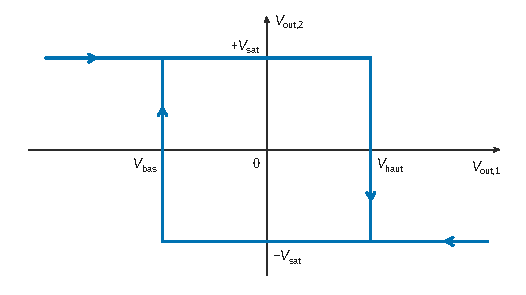
\includegraphics{figures/q15-cycle-hysteresis.pdf}
\caption*{Figure 1 --- Caractéristique du comparateur à hystérésis : cycle
inverseur parcouru dans le sens horaire, entre les seuils V\_bas et
V\_haut}
\end{figure}

\begin{piege}

Chaque seuil n'est actif que dans un état. Le graphe doit porter \(\pm V_{\mathrm{sat}}\), \(V_{\mathrm{haut}}\), \(V_{\mathrm{bas}}\) et le sens de parcours, sans quoi rien ne distingue un comparateur inverseur d'un non inverseur.

\end{piege}

\hypertarget{question-16}{%
\subsection{Question 16}\label{question-16}}

\begin{indication}{1}

Transistor bloqué : quel est le signe de \(V_{BE}\), donc celui de \(V_{\mathrm{out},2}\) ? Quel seuil est alors actif ?

\end{indication}

\begin{indication}{2}

Quelle variation totale la rampe doit-elle parcourir avant le basculement ? Pour la suite, suivez la chaîne : ALI 4, \(V_{BE}\), transistor, \(R_4\).

\end{indication}

\hypertarget{solution-15}{%
\subsubsection{Solution}\label{solution-15}}

Le transistor est bloqué, donc \(V_{BE}<0\). Comme \(V_{BE}\) et \(V_{\mathrm{out},2}\) ont toujours le même signe, \(V_{\mathrm{out},2}=-V_{\mathrm{sat}}\). Le seuil actif est donc \(V_{\mathrm{bas}}\).

La condition initiale donne \(V_0=-V_{\mathrm{bas}}=V_{\mathrm{haut}}\). La rampe \(V_{\mathrm{haut}}-st\) atteint \(V_{\mathrm{bas}}\) lorsque \(st_1=2V_{\mathrm{haut}}\) :

\equationajustee{\boxed{t_1=\frac{2R_7}{R_6+R_7}\cdot\frac{R_1C_1(R_2+R_3)}{R_2}\cdot\frac{V_{\mathrm{sat}}}{V_{\mathrm{in},1}}}}

Alors l'ALI 4 bascule à \(+V_{\mathrm{sat}}\) et \(V_{BE}\) devient positive. Le transistor passe en phase active : \(C\) est relié à \(E\), donc à la masse.

La résistance \(R_4\) dérive le courant

\equationajustee{\frac{V_{A_1}}{R_4}=\frac{R_3V_{\mathrm{in},1}}{R_4(R_2+R_3)}}

prélevé sur celui qui chargeait \(C_1\). Si \(R_4\) est assez petite, le courant dans \(C_1\) s'inverse et \(V_{\mathrm{out},1}\) se met à croître.

\begin{piege}

La rampe va du seuil haut au seuil bas : elle parcourt \(2V_{\mathrm{haut}}\) et non \(V_{\mathrm{haut}}\).

\end{piege}

\hypertarget{question-17}{%
\subsection{Question 17}\label{question-17}}

\begin{indication}{1}

Même loi des nœuds qu'en Q14, avec une branche supplémentaire vers la masse. \(V_{A_1}\) a-t-il changé ?

\end{indication}

\begin{indication}{2}

« Symétrique » : comparez les valeurs absolues des deux pentes.

\end{indication}

\hypertarget{solution-16}{%
\subsubsection{Solution}\label{solution-16}}

Pour \(t>t_1\), le transistor est passant et l'ALI 3 reste en régime linéaire, donc \(V_{A_1}=\dfrac{R_3}{R_2+R_3}V_{\mathrm{in},1}\) n'a pas changé. La loi des nœuds en \(A_1\) s'écrit

\equationajustee{\frac{V_{\mathrm{in},1}-V_{A_1}}{R_1}=\frac{V_{A_1}}{R_4}-C_1\frac{\mathrm{d}V_{\mathrm{out},1}}{\mathrm{d}t}}

d'où

\equationajustee{\frac{\mathrm{d}V_{\mathrm{out},1}}{\mathrm{d}t}=\frac{V_{\mathrm{in},1}}{C_1(R_2+R_3)}\Big(\frac{R_3}{R_4}-\frac{R_2}{R_1}\Big)}

\equationajustee{\boxed{V_{\mathrm{out},1}(t)=V_{\mathrm{bas}}+\frac{V_{\mathrm{in},1}}{C_1(R_2+R_3)}\Big(\frac{R_3}{R_4}-\frac{R_2}{R_1}\Big)(t-t_1)}}

Les oscillations sont symétriques si la pente montante est l'opposée de la pente descendante, \(+s\) : \(\dfrac{R_3}{R_4}-\dfrac{R_2}{R_1}=\dfrac{R_2}{R_1}\), soit

\equationajustee{\boxed{R_4=\frac{R_1R_3}{2R_2}}}

La pente est alors bien positive. \(V_{\mathrm{out},1}\) est un triangle symétrique et \(V_{\mathrm{out},2}\) un créneau de rapport cyclique \(1/2\).

\begin{piege}

Le courant \(V_{A_1}/R_4\) part vers la masse et se \textbf{retranche} du courant de charge. Une erreur de signe à cet endroit fait disparaître le facteur 2 de \(R_4\).

\end{piege}

\hypertarget{question-18}{%
\subsection{Question 18}\label{question-18}}

\begin{indication}{1}

Avec la condition de symétrie, les deux demi-périodes sont égales. Quel intervalle de tension chaque rampe parcourt-elle si \(R_6=R_7\) ?

\end{indication}

\hypertarget{solution-17}{%
\subsubsection{Solution}\label{solution-17}}

Avec \(R_6=R_7\), \(V_{\mathrm{haut}}=-V_{\mathrm{bas}}=V_{\mathrm{sat}}/2\). Chaque demi-période correspond au parcours de \(V_{\mathrm{sat}}\) à la pente \(s\) :

\equationajustee{\begin{aligned}
\frac T2&=\frac{V_{\mathrm{sat}}}{s}\\
&=\frac{R_1C_1(R_2+R_3)}{R_2}\frac{V_{\mathrm{sat}}}{V_{\mathrm{in},1}}
\end{aligned}}

d'où

\equationajustee{\boxed{f=\frac1{2R_1C_1}\,\frac{R_2}{R_2+R_3}\,\frac{V_{\mathrm{in},1}}{V_{\mathrm{sat}}}}}

La fréquence est proportionnelle à \(V_{\mathrm{in},1}\) : c'est l'hypothèse posée dès Q1. Contrôle d'homogénéité : \(R_1C_1\) est un temps, les autres facteurs sont sans dimension.

\hypertarget{question-19}{%
\subsection{Question 19}\label{question-19}}

\begin{indication}{1}

Alignez deux chronogrammes l'un sous l'autre : à quels instants le créneau bascule-t-il par rapport aux sommets du triangle ?

\end{indication}

\hypertarget{solution-18}{%
\subsubsection{Solution}\label{solution-18}}

Sur \([0,T/2]\), on a \(V_{\mathrm{out},2}=-V_{\mathrm{sat}}\). Pendant ce temps, \(V_{\mathrm{out},1}\) descend linéairement de \(+V_{\mathrm{sat}}/2\) à \(-V_{\mathrm{sat}}/2\).

Sur \([T/2,T]\), \(V_{\mathrm{out},2}=+V_{\mathrm{sat}}\) et \(V_{\mathrm{out},1}\) remonte.

\(V_{\mathrm{out},1}\) est donc un \textbf{triangle} symétrique d'amplitude crête \(V_{\mathrm{sat}}/2=7{,}5\ \mathrm{V}\). \(V_{\mathrm{out},2}\) est un \textbf{créneau} \(\pm15\ \mathrm{V}\) de rapport cyclique \(1/2\), qui bascule exactement aux sommets du triangle.

\begin{figure}[H]
\centering
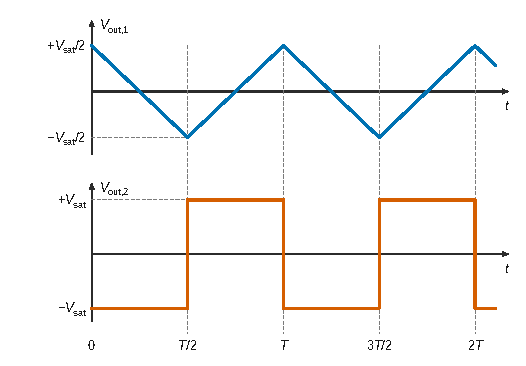
\includegraphics{figures/q19-chronogrammes-vco.pdf}
\caption*{Figure 2 --- Chronogrammes de l'oscillateur : triangle V\_out,1 entre
±V\_sat/2 et créneau V\_out,2 = ±V\_sat, qui bascule aux sommets du
triangle}
\end{figure}

\begin{jury}

Un chronogramme se lit grâce à ses axes nommés, ses valeurs remarquables et l'alignement vertical des deux tracés. Les valeurs à porter sont \(\pm V_{\mathrm{sat}}\) et \(\pm V_{\mathrm{sat}}/2\) en ordonnée. En abscisse, on marque \(T/2\) et \(T\).

\end{jury}

\hypertarget{question-20}{%
\subsection{Question 20}\label{question-20}}

\begin{indication}{1}

La vitesse de balayage borne la dérivée de la tension de sortie. Quel ALI est en contre-réaction, et quelle est la pente de sa sortie en fonction de \(f\) ?

\end{indication}

\begin{indication}{2}

Pour le commentaire, comparez la borne obtenue à des fréquences musicales (La\(_0\), limite de l'audition) et pensez au comparateur.

\end{indication}

\hypertarget{solution-19}{%
\subsubsection{Solution}\label{solution-19}}

La vitesse de balayage \(\sigma=0{,}3\ \mathrm{V\cdot\mu s^{-1}}\) est la valeur maximale de \(|\mathrm{d}V_s/\mathrm{d}t|\) que peut atteindre la sortie d'un ALI réel, quel que soit le signal d'entrée. C'est une limitation non linéaire de l'étage de sortie, absente du modèle idéal. Elle déforme les signaux trop rapides : les pentes sont écrêtées et les fronts deviennent des rampes.

L'ALI 3, en contre-réaction, délivre un triangle qui parcourt \(V_{\mathrm{sat}}\) en \(T/2\), de pente \(s=2fV_{\mathrm{sat}}\). Il faut \(2fV_{\mathrm{sat}}\leqslant\sigma\) :

\equationajustee{\begin{aligned}
f&\leqslant\frac{\sigma}{2V_{\mathrm{sat}}}\\
&=\frac{0{,}3\times10^6}{2\times15}\\
&=\boxed{1{,}0\times10^4\ \mathrm{Hz}}
\end{aligned}}

\emph{Commentaire.} Le La\(_0\) vaut \(55\ \mathrm{Hz}\). \(10\ \mathrm{kHz}\) correspond à environ 7,5 octaves au-dessus et couvre le fondamental de toutes les notes d'un clavier, mais pas tout le domaine audible (\(20\ \mathrm{kHz}\)) ni les harmoniques des notes aiguës, qui donnent le timbre.

Le comparateur (ALI 4) est lui aussi limité : un front de \(2V_{\mathrm{sat}}=30\ \mathrm{V}\) dure \(100\ \mu\mathrm{s}\). Cette durée n'est négligeable devant \(T/2\) que pour \(f\ll5\ \mathrm{kHz}\). Au-delà, le créneau devient trapézoïdal et le fonctionnement s'écarte du modèle.

\begin{methode}

Vitesse de balayage : on calcule la pente maximale du signal de sortie (pour un triangle, amplitude crête à crête divisée par la demi-période ; pour une sinusoïde, \(2\pi fV_m\)) et on la compare à \(\sigma\).

\end{methode}

\hypertarget{partie-b-contruxf4le-de-tempuxe9rature-au-sein-dun-synthuxe9tiseur-analogique}{%
\section{Partie B --- Contrôle de température au sein d'un synthétiseur analogique}\label{partie-b-contruxf4le-de-tempuxe9rature-au-sein-dun-synthuxe9tiseur-analogique}}

C'est le problème classique de l'ailette : bilan d'énergie sur une tranche, équation différentielle du second ordre, conditions aux limites, profil de température et flux évacué, puis rendement. Les données numériques servent surtout à évaluer \(m\ell\). C'est ce nombre qui tranche Q24 et explique pourquoi la forme de l'ailette compte peu en Q31.

\hypertarget{question-21}{%
\subsection{Question 21}\label{question-21}}

\begin{indication}{1}

Quelles faces de la tranche \([x,x+\mathrm{d}x]\) sont en contact avec l'air ? Les sections droites en font-elles partie ?

\end{indication}

\begin{indication}{2}

« Précisément » : n'oubliez pas les chants d'épaisseur \(e\), quitte à les négliger ensuite en le justifiant.

\end{indication}

\hypertarget{solution-20}{%
\subsubsection{Solution}\label{solution-20}}

La tranche est un pavé \(\mathrm{d}x\times L\times e\). Au contact de l'air se trouvent les deux grandes faces (aire \(L\,\mathrm{d}x\) chacune) et les deux chants (aire \(e\,\mathrm{d}x\) chacun). Les sections droites en \(x\) et en \(x+\mathrm{d}x\) sont en contact avec le reste de l'ailette. La loi de Newton donne la puissance cédée à l'air :

\equationajustee{\boxed{\begin{aligned}
\delta P&=2h(L+e)\big(T(x,t)-T_a\big)\,\mathrm{d}x\\
&\simeq2hL\big(T(x,t)-T_a\big)\,\mathrm{d}x\quad(e\ll L)
\end{aligned}}}

Elle est positive puisque \(T>T_a\).

\hypertarget{question-22}{%
\subsection{Question 22}\label{question-22}}

\begin{indication}{1}

Premier principe en régime stationnaire pour la tranche : ce qui entre par conduction en \(x\) ressort par conduction en \(x+\mathrm{d}x\) et par les faces.

\end{indication}

\begin{indication}{2}

Loi de Fourier avec l'aire de la section droite (\(Le\)), puis développement au premier ordre en \(\mathrm{d}x\).

\end{indication}

\hypertarget{solution-21}{%
\subsubsection{Solution}\label{solution-21}}

Le flux conductif à travers la section d'abscisse \(x\) vaut \(\Phi(x)=-\lambda Le\,\dfrac{\mathrm{d}T}{\mathrm{d}x}\). En régime stationnaire, rien ne s'accumule dans la tranche :

\equationajustee{0=\Phi(x)-\Phi(x+\mathrm{d}x)-2h(L+e)(T-T_a)\,\mathrm{d}x}

avec

\equationajustee{\Phi(x)-\Phi(x+\mathrm{d}x)=\lambda Le\,\frac{{\mathrm{d}}^2T}{\mathrm{d}x^2}\,\mathrm{d}x}

En divisant par \(\lambda Le\,\mathrm{d}x\) :

\equationajustee{\frac{{\mathrm{d}}^2T}{\mathrm{d}x^2}-m^2T=-m^2T_a}

avec

\equationajustee{\begin{aligned}
m^2&=\frac{2h(L+e)}{\lambda Le}\\
&\underset{e\ll L}{\simeq}\frac{2h}{\lambda e}
\end{aligned}}

d'où

\equationajustee{\boxed{m=\sqrt{\frac{2h}{\lambda e}}}}

\(m\) est bien l'inverse d'une longueur. A.N. :

\equationajustee{\begin{aligned}
m&=\sqrt{\frac{2\times50}{215\times2{,}0\times10^{-3}}}\\
&=15{,}2\ \mathrm{m^{-1}}
\end{aligned}}

soit \(1/m=6{,}6\ \mathrm{cm}\). Les données \(\rho\) et \(c\) ne servent pas : elles ne fixeraient que la durée du régime transitoire.

\begin{methode}

Bilan sur une tranche : (1) choisir le système ; (2) écrire chaque flux avec sa surface ; (3) développer \(\Phi(x+\mathrm{d}x)\) au premier ordre ; (4) simplifier par \(\mathrm{d}x\). L'hypothèse « \(T\) uniforme sur une section » justifie le modèle unidimensionnel.

\end{methode}

\hypertarget{question-23}{%
\subsection{Question 23}\label{question-23}}

\begin{indication}{1}

Que signifie un contact thermique parfait à une interface ?

\end{indication}

\hypertarget{solution-22}{%
\subsubsection{Solution}\label{solution-22}}

Le contact avec le transistor, à \(T_1\) constante, est parfait : il n'y a pas de résistance de contact et la température est continue. Donc \(\boxed{T(0)=T_1}\).

\hypertarget{question-24}{%
\subsection{Question 24}\label{question-24}}

\begin{indication}{1}

Traduisez chaque hypothèse : comportement à grande distance, flux de Fourier nul, égalité entre flux conductif et flux conducto-convectif sur la section terminale.

\end{indication}

\begin{indication}{2}

Pour juger du réalisme, calculez \(m\ell\) avec les dimensions données plus loin, et comparez la surface d'extrémité à la surface latérale.

\end{indication}

\hypertarget{solution-23}{%
\subsubsection{Solution}\label{solution-23}}

La solution générale s'écrit \(T=T_a+A{\mathrm{e}}^{-mx}+B{\mathrm{e}}^{mx}\).

\begin{itemize}
\tightlist
\item
  \textbf{Hypothèse 1} (\(m\ell\gg1\)) : l'ailette se comporte comme si elle était infinie et la température doit rester bornée, d'où \(B=0\) et \(\boxed{T(\ell)\simeq T_a}\).
\item
  \textbf{Hypothèse 2} : flux de Fourier nul en bout d'ailette, \(\boxed{\dfrac{\mathrm{d}T}{\mathrm{d}x}(\ell)=0}\) (extrémité calorifugée).
\item
  \textbf{Hypothèse 3} : le flux conductif arrivant sur la section terminale est évacué par conducto-convection, \(-\lambda Le\,T'(\ell)=hLe\,(T(\ell)-T_a)\), soit \(\boxed{-\lambda\dfrac{\mathrm{d}T}{\mathrm{d}x}(\ell)=h\big(T(\ell)-T_a\big)}\).
\end{itemize}

\textbf{L'hypothèse 3 est la plus réaliste} : rien n'isole l'extrémité, baignée par le même air que le reste. L'hypothèse 1 est ici fausse : \(m\ell=15{,}2\times0{,}015=0{,}23\ll1\). L'hypothèse 2 est une bonne approximation de la 3, car la surface d'extrémité \(Le\) ne représente que \(e/(2\ell)\approx7\ \%\) de la surface latérale \(2L\ell\). L'énoncé le confirme plus loin : il suffit d'allonger l'ailette de \(e/2\) pour passer de l'une à l'autre.

\begin{piege}

Choisir l'hypothèse 2 « parce que c'est celle qu'on utilise ensuite » confond commodité de calcul et réalisme physique. Et un rejet de l'hypothèse 1 s'appuie sur la valeur de \(m\ell\), pas sur une impression.

\end{piege}

\hypertarget{question-25}{%
\subsection{Question 25}\label{question-25}}

\begin{indication}{1}

Que devient le terme en \({\mathrm{e}}^{+mx}\) si la température doit rester bornée ?

\end{indication}

\hypertarget{solution-24}{%
\subsubsection{Solution}\label{solution-24}}

\(B=0\), et \(T(0)=T_1\) donne \(A=T_1-T_a\) :

\equationajustee{\boxed{T(x)=T_a+(T_1-T_a)\,{\mathrm{e}}^{-mx}}}

\equationajustee{\boxed{\widetilde T(x)={\mathrm{e}}^{-mx}}}

Tracé (figure 3) : \(\widetilde T\) décroît de 1 en \(x=0\) vers 0. La tangente à l'origine, de pente \(-m\), coupe l'axe en \(x=1/m\approx6{,}6\ \mathrm{cm}\), la longueur caractéristique de pénétration de la chaleur.

\begin{figure}[H]
\centering
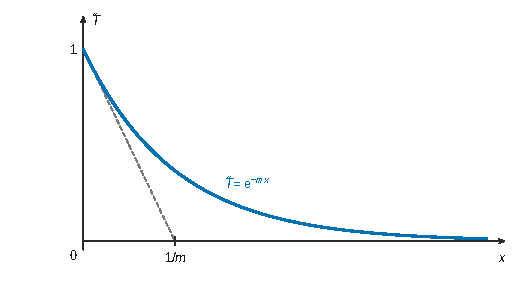
\includegraphics{figures/q25-profil-ailette.pdf}
\caption*{Figure 3 --- Profil de température réduit de l'ailette semi-infinie, T̃ =
exp(−mx), et sa tangente à l'origine qui coupe l'axe en x = 1/m}
\end{figure}

\hypertarget{question-26}{%
\subsection{Question 26}\label{question-26}}

\begin{indication}{1}

Écrivez la solution générale avec des fonctions hyperboliques de \(m(\ell-x)\) : l'une d'elles a une dérivée nulle en \(x=\ell\).

\end{indication}

\hypertarget{solution-25}{%
\subsubsection{Solution}\label{solution-25}}

\(\theta=T-T_a\) vérifie \(\theta''=m^2\theta\), et on l'écrit \(\theta=P\cosh(m(\ell-x))+Q\sinh(m(\ell-x))\). On a \(\theta'(\ell)=-mQ=0\), donc \(Q=0\). Puis \(\theta(0)=P\cosh(m\ell)=T_1-T_a\), d'où

\equationajustee{\boxed{\widetilde T(x)=\frac{\cosh\big(m(\ell-x)\big)}{\cosh(m\ell)}}}

Vérifications : \(\widetilde T(0)=1\) et \(\widetilde T'(\ell)=0\). Numériquement, \(\widetilde T(\ell)=1/\cosh(0{,}229)=0{,}974\) : l'ailette est presque isotherme.

\begin{methode}

Centrer la solution sur l'extrémité où porte la condition de flux, avec \(\cosh(m(\ell-x))\) et \(\sinh(m(\ell-x))\), annule une constante immédiatement et évite un système de deux équations.

\end{methode}

\hypertarget{question-27}{%
\subsection{Question 27}\label{question-27}}

\begin{indication}{1}

En régime stationnaire, avec une extrémité qui n'évacue rien, d'où vient toute l'énergie évacuée par les faces ?

\end{indication}

\begin{indication}{2}

Calculez le flux conductif entrant en \(x=0\) par la loi de Fourier, ou intégrez les pertes latérales : les deux voies doivent concorder.

\end{indication}

\hypertarget{solution-26}{%
\subsubsection{Solution}\label{solution-26}}

Il n'y a ni accumulation ni flux en \(x=\ell\) : tout le flux entré par la base est évacué par les faces. Donc \(\Phi=-\lambda Le\,T'(0)\), avec \(T'(0)=-m(T_1-T_a)\tanh(m\ell)\) :

\equationajustee{\boxed{\begin{aligned}
\Phi&=\lambda Le\,m\,(T_1-T_a)\tanh(m\ell)\\
&=\frac{2hL}{m}(T_1-T_a)\tanh(m\ell)
\end{aligned}}}

La seconde forme utilise \(\lambda e=2h/m^2\). Vérification par intégration :

\equationajustee{\int_0^\ell2hL\,\theta\,\mathrm{d}x=\frac{2hL(T_1-T_a)}{\cosh(m\ell)}\cdot\frac{\sinh(m\ell)}{m}}

c'est le même résultat. A.N. : \(\Phi\approx2{,}9\times10^{-2}\ \mathrm{W\cdot K^{-1}}\times(T_1-T_a)\), soit environ \(0{,}9\ \mathrm{W}\) pour un écart de \(30\ \mathrm{K}\).

\hypertarget{question-28}{%
\subsection{Question 28}\label{question-28}}

\begin{indication}{1}

Comment varie la température le long de l'ailette ? Quel est l'écart de température qui « pilote » la loi de Newton en chaque point ?

\end{indication}

\hypertarget{solution-27}{%
\subsubsection{Solution}\label{solution-27}}

L'ailette perd de la chaleur tout au long du trajet depuis sa base : sa température décroît avec \(x\) (\(\widetilde T<1\) pour \(x>0\)). L'écart local \(T(x)-T_a\), qui commande la loi de Newton, est donc partout inférieur à \(T_1-T_a\), et chaque élément de surface échange moins que s'il était à \(T_1\).

Donc \(\boxed{\Phi<\Phi_u}\). L'égalité correspondrait à une ailette de conductivité infinie (\(m\to0\)).

\begin{piege}

« Sans calcul » : l'argument attendu est physique (le profil décroît), pas l'inégalité \(\tanh u<u\).

\end{piege}

\hypertarget{question-29}{%
\subsection{Question 29}\label{question-29}}

\begin{indication}{1}

Quelles propriétés caractérisent un rendement ? Vérifiez-les sur \(\eta\).

\end{indication}

\hypertarget{solution-28}{%
\subsubsection{Solution}\label{solution-28}}

\(\eta\) est le quotient de deux puissances, donc sans dimension, et il est compris entre 0 et 1 d'après Q28. Il compare ce que l'ailette évacue réellement à ce qu'elle évacuerait au mieux, à surface et conditions extérieures identiques : c'est bien un rendement. La « perte » qu'il traduit n'est pas une énergie dissipée : elle vient de la résistance thermique interne de l'ailette, qui empêche l'extrémité de rester à \(T_1\).

\hypertarget{question-30}{%
\subsection{Question 30}\label{question-30}}

\begin{indication}{1}

Calculez \(\Phi_u\) avec la même surface d'échange que celle utilisée pour \(\Phi\).

\end{indication}

\begin{indication}{2}

Éliminez \(\lambda e\) grâce à l'expression de \(m^2\).

\end{indication}

\hypertarget{solution-29}{%
\subsubsection{Solution}\label{solution-29}}

\(\Phi_u=2hL\ell(T_1-T_a)\) : ce sont les deux grandes faces, l'extrémité étant exclue par l'hypothèse 2. En divisant le résultat de Q27, puis en utilisant \(\lambda e=2h/m^2\) :

\equationajustee{\begin{aligned}
\eta&=\frac{\lambda Le\,m\tanh(m\ell)}{2hL\ell}\\
&=\frac{\lambda e\,m}{2h\ell}\tanh(m\ell)\\
&=\boxed{\frac{\tanh(m\ell)}{m\ell}}
\end{aligned}}

Limites : \(\eta\to1\) quand \(m\ell\to0\) (ailette quasi isotherme). À l'inverse, \(\eta\sim1/(m\ell)\to0\) quand \(m\ell\to\infty\) (allonger encore l'ailette n'apporte rien).

\begin{methode}

Les deux cas limites d'un résultat (\(m\ell\to0\) et \(m\ell\to\infty\)) se vérifient en deux lignes et valident la formule.

\end{methode}

\hypertarget{question-31}{%
\subsection{Question 31}\label{question-31}}

\begin{indication}{1}

Les trois rendements ne dépendent que de \(m\ell\) (ou de \(m\ell_c\) pour la rectangulaire, qui échange aussi par son extrémité). Calculez ces nombres avec les dimensions maximales données.

\end{indication}

\begin{indication}{2}

Pour l'ailette triangulaire, le graphe du formulaire se lit en \(x=2m\ell\) et non en \(m\ell\). Avant de conclure, vérifiez que les trois profils offrent la même surface d'échange.

\end{indication}

\hypertarget{solution-30}{%
\subsubsection{Solution}\label{solution-30}}

Valeurs utiles : \(m=15{,}2\ \mathrm{m^{-1}}\) et \(m\ell=0{,}229\). Pour les deux autres profils, \(m\ell_c=m(\ell+e/2)=0{,}244\) et \(2m\ell=0{,}457\).

\begin{longtable}[]{@{}
  >{\raggedright\arraybackslash}p{(\columnwidth - 4\tabcolsep) * \real{0.3333}}
  >{\raggedright\arraybackslash}p{(\columnwidth - 4\tabcolsep) * \real{0.3333}}
  >{\raggedright\arraybackslash}p{(\columnwidth - 4\tabcolsep) * \real{0.3333}}@{}}
\toprule\noalign{}
\begin{minipage}[b]{\linewidth}\raggedright
Ailette
\end{minipage} & \begin{minipage}[b]{\linewidth}\raggedright
Calcul
\end{minipage} & \begin{minipage}[b]{\linewidth}\raggedright
\(\eta\)
\end{minipage} \\
\midrule\noalign{}
\endhead
\bottomrule\noalign{}
\endlastfoot
rectangulaire & \(\tanh(0{,}244)/0{,}244\) & \(0{,}981\) \\
triangulaire & \(I_1/I_0\) lu en \(0{,}457\) : \(\approx0{,}223\), puis \(0{,}223/0{,}229\) & \(0{,}975\) \\
parabolique & \(2/\big(1+\sqrt{0{,}209+1}\big)\) & \(0{,}953\) \\
\end{longtable}

Les trois profils ont les mêmes dimensions \(L\), \(\ell\), \(e\). La face inclinée de l'ailette triangulaire a une aire \(2L\sqrt{\ell^2+e^2/4}\), égale à \(2L\ell\) à \(0{,}2\ \%\) près, et de même pour le profil parabolique.

Les \(\Phi_u\) sont donc pratiquement égaux et les flux se classent comme les rendements :

\equationajustee{\boxed{\text{l'ailette rectangulaire dissipe le plus}\ (\eta\approx0{,}98)}}

Les écarts sont faibles, parce que \(m\ell\ll1\) : l'ailette est courte et quasi isotherme, et la forme du profil compte peu. L'ailette triangulaire contient deux fois moins d'aluminium pour \(0{,}6\ \%\) de flux en moins. Rapportée à la masse ou au coût, elle serait la plus avantageuse, ce qui rejoint les « raisons économiques » évoquées par l'énoncé.

\begin{piege}

L'argument de la fonction de Bessel est \(2m\ell\), et l'axe du graphe s'arrête justement à \(0{,}50\). Comparer des rendements sans vérifier que les surfaces sont comparables ne permet pas de conclure sur les flux.

\end{piege}

\hypertarget{question-32}{%
\subsection{Question 32}\label{question-32}}

\begin{indication}{1}

De quoi dépend le coefficient \(h\) ? Pensez à la couche limite thermique au voisinage de la paroi.

\end{indication}

\begin{indication}{2}

Quel nombre sans dimension distingue les régimes d'écoulement, et quel régime renouvelle le mieux l'air au contact de l'ailette ?

\end{indication}

\hypertarget{solution-31}{%
\subsubsection{Solution}\label{solution-31}}

Il faut privilégier une \textbf{convection forcée en écoulement turbulent} : un ventilateur qui impose un nombre de Reynolds élevé. Le coefficient \(h\) mesure l'efficacité du transfert dans la couche d'air proche de la paroi, où la chaleur traverse une couche limite d'épaisseur \(\delta\) par diffusion : \(h\sim\lambda_{\mathrm{air}}/\delta\). Une vitesse élevée amincit cette couche limite. Le régime turbulent ajoute un brassage qui renouvelle sans cesse l'air chaud au contact de l'ailette. En convection naturelle, au contraire, l'air se déplace lentement sous l'effet de la poussée d'Archimède et \(h\) reste faible.

Augmenter \(h\) fait croître \(m\propto\sqrt h\) et baisser légèrement \(\eta\). Mais le flux \(\Phi=\eta\,h\,2L\ell\,(T_1-T_a)\) augmente : pour \(m\ell\) petit, \(\eta\) ne diminue qu'au second ordre.

\begin{piege}

Le \(\lambda\) qui intervient dans \(h\) est celui de l'air, pas celui de l'aluminium.

\end{piege}

\hypertarget{partie-c-protection-par-couches-minces-de-composuxe9s-du-silicium}{%
\section{Partie C --- Protection par couches minces de composés du silicium}\label{partie-c-protection-par-couches-minces-de-composuxe9s-du-silicium}}

La sous-partie I est de la thermochimie (grandeurs standard de réaction, constante d'équilibre, température de fin de réaction adiabatique) suivie de cinétique (exploitation de mesures thermogravimétriques, ordre 0, loi d'Arrhenius). La sous-partie II est un modèle de transport en série : trois flux égaux, trois « résistances », une équation différentielle à variables séparables, puis deux régimes asymptotiques.

\hypertarget{question-33}{%
\subsection{Question 33}\label{question-33}}

\begin{indication}{1}

Équilibrez avec un coefficient 1 pour \(\mathrm{Si_3N_4}\). Que valent les enthalpies standard de formation des corps simples ?

\end{indication}

\begin{indication}{2}

Calculez \(\Delta_rH^\circ\) et \(\Delta_rS^\circ\). Déduisez-en \(\Delta_rG^\circ\), puis \(K^\circ\).

La constante \(R\) se déduit des données (\(k_B\) et \(N_A\)). Donnez un critère chiffré de réaction quantitative.

\end{indication}

\hypertarget{solution-32}{%
\subsubsection{Solution}\label{solution-32}}

\equationajustee{\boxed{3\,\mathrm{Si(s)}+2\,\mathrm{N_2(g)}=\mathrm{Si_3N_4(s)}}}

C'est la réaction de formation de \(\mathrm{Si_3N_4}\) : \(\Delta_rH^\circ=\Delta_fH^\circ(\mathrm{Si_3N_4})=-828\ \mathrm{kJ\cdot mol^{-1}}\). De plus

\equationajustee{\begin{aligned}
\Delta_rS^\circ&=113-3\times18{,}8-2\times192\\
&=-327{,}4\ \mathrm{J\cdot K^{-1}\cdot mol^{-1}}
\end{aligned}}

Ce signe est cohérent : deux moles de gaz disparaissent. On en déduit

\equationajustee{\begin{aligned}
\Delta_rG^\circ(298)&=-828\times10^3+298\times327{,}4\\
&=-7{,}30\times10^5\ \mathrm{J\cdot mol^{-1}}
\end{aligned}}

Avec \(R=k_BN_A=8{,}31\ \mathrm{J\cdot K^{-1}\cdot mol^{-1}}\) :

\equationajustee{\begin{aligned}
\ln K^\circ&=-\frac{\Delta_rG^\circ}{RT}\\
&=\frac{7{,}30\times10^5}{8{,}31\times298}\\
&=295
\end{aligned}}

\equationajustee{\boxed{K^\circ\approx10^{128}}}

\(K^\circ\gg10^4\) : à l'équilibre, \(K^\circ=(P^\circ/P_{\mathrm{N_2}})^2\) impose \(P_{\mathrm{N_2}}\approx10^{-64}\ \mathrm{bar}\), une valeur nulle en pratique. \textbf{La réaction est quantitative à \(298\ \mathrm{K}\).}

\begin{piege}

Pièges classiques : mélanger kJ et J dans \(\Delta_rH^\circ-T\Delta_rS^\circ\), oublier les coefficients 3 et 2 dans \(\Delta_rS^\circ\), ou prendre pour un oubli de l'énoncé la colonne vide des \(\Delta_fH^\circ\) (elle vaut zéro pour les corps simples).

\end{piege}

\hypertarget{question-34}{%
\subsection{Question 34}\label{question-34}}

\begin{indication}{1}

Réacteur calorifugé et isobare : quelle fonction d'état est conservée ? Construisez un chemin fictif en deux étapes.

\end{indication}

\begin{indication}{2}

Après la réaction totale, quelles espèces restent à échauffer ? Pour conclure, confrontez le résultat aux températures de fusion données, et à la température au-delà de laquelle \(\Delta_rG^\circ\) change de signe.

\end{indication}

\hypertarget{solution-33}{%
\subsubsection{Solution}\label{solution-33}}

Le réacteur est calorifugé et isobare : \(\Delta H=Q_P=0\). On suit un chemin fictif en deux étapes.

\begin{enumerate}
\def\labelenumi{\arabic{enumi}.}
\tightlist
\item
  Réaction totale à \(298\ \mathrm{K}\), pour \(\xi=1\ \mathrm{mol}\) : \(\Delta H_1=\Delta_rH^\circ\).
\item
  Échauffement du seul produit, puisqu'il ne reste aucun réactif (proportions stœchiométriques, réaction quantitative) : \(\Delta H_2=C_{pm}(\mathrm{Si_3N_4})(T_f-298)\).
\end{enumerate}

La condition \(\Delta H_1+\Delta H_2=0\) donne

\equationajustee{\begin{aligned}
T_f&=298+\frac{828\times10^3}{99{,}5}\\
&\approx\boxed{8{,}6\times10^3\ \mathrm{K}}
\end{aligned}}

\emph{Conclusion.} Ce résultat est irréaliste et sort du domaine de validité du modèle. Il dépasse largement \(T_{\mathrm{fus}}(\mathrm{Si})=1687\ \mathrm{K}\) et \(T_{\mathrm{fus}}(\mathrm{Si_3N_4})=2173\ \mathrm{K}\) (les changements d'état ne sont pas pris en compte). Il dépasse aussi la température d'inversion \(T_i=\Delta_rH^\circ/\Delta_rS^\circ\approx2{,}5\times10^3\ \mathrm{K}\), au-delà de laquelle \(\Delta_rG^\circ>0\) : la réaction cesserait d'être quantitative et le nitrure se décomposerait.

Retenons que la réaction est \textbf{très exothermique} : en réacteur calorifugé, elle s'emballerait et détruirait le produit. Il faut évacuer la chaleur, ce que fera le réacteur isotherme de la suite.

\begin{methode}

Température de fin de réaction adiabatique : on écrit \(\Delta H=0\) sur un chemin fictif (réaction à \(T_i\), puis échauffement de \textbf{tout ce qui est présent en fin de réaction}). On confronte ensuite \(T_f\) aux changements d'état et à la température d'inversion.

\end{methode}

\hypertarget{question-35}{%
\subsection{Question 35}\label{question-35}}

\begin{indication}{1}

Que « voit » la balance ? Reliez la prise de masse à l'avancement, puis la masse de silicium consommée au même avancement.

\end{indication}

\begin{indication}{2}

Pour relier \(W^0_{\mathrm{Si}}\) à \(W^0\), le tableau de composition donne le titre massique en silicium.

\end{indication}

\hypertarget{solution-34}{%
\subsubsection{Solution}\label{solution-34}}

Pour un avancement \(\xi\) : la masse de silicium consommée vaut \(\Delta W_{\mathrm{Si}}=3\xi M_{\mathrm{Si}}\). Le solide gagne l'azote fixé, \(\Delta W=4\xi M_{\mathrm{N}}\), en supposant que seul le silicium réagit et que le gaz n'apporte pas d'autre variation de masse. Enfin \(W^0_{\mathrm{Si}}=0{,}6856\,W^0\). D'où

\equationajustee{\begin{aligned}
\alpha&=\frac{3\xi M_{\mathrm{Si}}}{0{,}6856\,W^0}\\
&=\frac{3M_{\mathrm{Si}}}{4M_{\mathrm{N}}\times0{,}6856}\cdot\frac{\Delta W}{W^0}
\end{aligned}}

donc

\equationajustee{\begin{aligned}
\beta&=\frac{3\times28{,}1}{4\times14{,}0\times0{,}6856}\\
&=\boxed{2{,}20}
\end{aligned}}

Contrôle : pour \(\alpha=1\), la prise de masse est de \(1/2{,}20=45\ \%\). C'est cohérent avec \(M(\mathrm{Si_3N_4})/(3M_{\mathrm{Si}})=1{,}66\) et un titre en silicium de \(68{,}6\ \%\).

\begin{piege}

La balance mesure la masse d'azote fixée, pas celle du nitrure formé. Oublier le titre de \(68{,}56\ \%\) donne \(\beta=1{,}51\). Les autres colonnes du tableau ne servent pas.

\end{piege}

\hypertarget{question-36}{%
\subsection{Question 36}\label{question-36}}

\begin{indication}{1}

Comparez les courbes de la figure 11-a) à \(1400\) et \(1500\ ^\circ\mathrm{C}\). Une donnée du formulaire tombe précisément entre ces deux températures.

\end{indication}

\begin{indication}{2}

Pensez à l'état physique du réactif et à ce qui se forme à la surface des grains. Si vous invoquez la thermodynamique, chiffrez \(K^\circ\) à \(1500\ ^\circ\mathrm{C}\) pour vérifier que l'argument tient.

\end{indication}

\hypertarget{solution-35}{%
\subsubsection{Solution}\label{solution-35}}

À 1500 °C, le taux de nitruration plafonne vers 40 \%, contre environ 60 \% à 1350 et 1400 °C, alors même que la réaction démarre vite. Deux phénomènes peuvent l'expliquer :

\begin{enumerate}
\def\labelenumi{\arabic{enumi}.}
\tightlist
\item
  \textbf{La fusion du silicium} (\(T_{\mathrm{fus}}=1414\ ^\circ\mathrm{C}\), entre 1400 et \(1500\ ^\circ\mathrm{C}\)). Les grains fondent et coalescent, la surface de contact entre solide et gaz s'effondre, et le liquide se couvre de nitrure.
\item
  \textbf{La formation rapide d'une couche dense et passivante de \(\mathrm{Si_3N_4}\)} autour des grains. Elle fait obstacle à la diffusion de \(\mathrm{N_2}\) vers le silicium non converti. La forte exothermicité (\(-828\ \mathrm{kJ\cdot mol^{-1}}\)) l'aggrave : elle crée des surchauffes locales au-dessus de la consigne du four, qui accélèrent le frittage et la fusion.
\end{enumerate}

L'argument thermodynamique (réaction exothermique, donc \(K^\circ\) décroissant avec \(T\) selon la loi de van 't Hoff) va dans le même sens, mais pèse peu ici. Avec \(\Delta_rH^\circ\) et \(\Delta_rS^\circ\) supposés indépendants de la température :

\equationajustee{\begin{aligned}
\Delta_rG^\circ(1773\ \mathrm{K})&\approx-828+1773\times0{,}327\\
&\approx-2{,}5\times10^2\ \mathrm{kJ\cdot mol^{-1}}
\end{aligned}}

soit \(K^\circ\approx{\mathrm{e}}^{17}\) : la réaction reste favorable sous 1 bar de \(\mathrm{N_2}\).

\begin{piege}

Ne confondez pas la vitesse initiale, plus grande à \(1500\ ^\circ\mathrm{C}\), avec le taux final, plus faible. Et invoquer la loi de van 't Hoff sans chiffrer \(K^\circ\) risque de conclure trop vite.

\end{piege}

\hypertarget{question-37}{%
\subsection{Question 37}\label{question-37}}

\begin{indication}{1}

Que signifie un ordre 0 pour la vitesse \(\mathrm{d}\xi/\mathrm{d}t\) ? Reliez ensuite \(\alpha\) à \(\xi\) comme en Q35.

\end{indication}

\hypertarget{solution-36}{%
\subsubsection{Solution}\label{solution-36}}

À l'ordre 0, la vitesse molaire est indépendante des concentrations : \(\dfrac{\mathrm{d}\xi}{\mathrm{d}t}=k\), donc \(\xi=kt\). Comme \(\alpha=\dfrac{3M_{\mathrm{Si}}\xi}{W^0_{\mathrm{Si}}}\) :

\equationajustee{\boxed{\begin{aligned}
\alpha(t)&=\frac{3M_{\mathrm{Si}}}{W^0_{\mathrm{Si}}}\,k\,t\\
&=\frac{3M_{\mathrm{Si}}}{0{,}6856\,W^0}\,k\,t
\end{aligned}}}

C'est une droite passant par l'origine, ce que montre la figure 11-b). Ici \(k\) s'exprime en \(\mathrm{mol\cdot min^{-1}}\). L'énoncé impose la vitesse molaire parce qu'un lit de poudre traversé par un gaz n'a pas de volume réactionnel bien défini.

\hypertarget{question-38}{%
\subsection{Question 38}\label{question-38}}

\begin{indication}{1}

Formule, puis une ligne par grandeur avec son unité. L'unité du facteur préexponentiel dépend de celle de \(k\).

\end{indication}

\hypertarget{solution-37}{%
\subsubsection{Solution}\label{solution-37}}

\equationajustee{\boxed{k(T)=A\exp\Big(-\frac{E_a}{RT}\Big)}}

\begin{itemize}
\tightlist
\item
  \(k\) : constante de vitesse, ici en \(\mathrm{mol\cdot s^{-1}}\) (ordre 0, vitesse molaire) ;
\item
  \(A\) : facteur préexponentiel, de même unité que \(k\) ;
\item
  \(E_a\) : énergie d'activation, positive, en \(\mathrm{J\cdot mol^{-1}}\) ;
\item
  \(R=8{,}31\ \mathrm{J\cdot K^{-1}\cdot mol^{-1}}\) : constante des gaz parfaits ;
\item
  \(T\) : température absolue, en K.
\end{itemize}

Forme exploitable : \(\ln k=\ln A-\dfrac{E_a}{R}\cdot\dfrac1T\), affine en \(1/T\).

\hypertarget{question-39}{%
\subsection{Question 39}\label{question-39}}

\begin{indication}{1}

Mesurez la pente de chaque série de la figure 11-b), puis passez de la pente de \(\alpha(t)\) à \(k\) grâce à Q37.

\end{indication}

\begin{indication}{2}

Tracez \(\ln k\) en fonction de \(1/T\) (températures en kelvins) : la pente et l'ordonnée à l'origine donnent les deux paramètres. Discutez la précision obtenue.

\end{indication}

\hypertarget{solution-38}{%
\subsubsection{Solution}\label{solution-38}}

Les trois séries sont alignées et passent par l'origine. À \(t=30\ \mathrm{min}\), on lit respectivement 13,8 \%, 20,7 \% et 25,2 \% pour \(\alpha\). Les pentes valent donc \(a=0{,}460\), \(0{,}690\) et \(0{,}840\ \%\cdot\mathrm{min^{-1}}\).

On passe à \(k\) par \(k=\dfrac{W^0_{\mathrm{Si}}}{3M_{\mathrm{Si}}}a\), où \(W^0_{\mathrm{Si}}=0{,}6856\times834=571{,}8\ \mathrm{g}\) :

\begin{longtable}[]{@{}
  >{\raggedright\arraybackslash}p{(\columnwidth - 6\tabcolsep) * \real{0.2500}}
  >{\raggedright\arraybackslash}p{(\columnwidth - 6\tabcolsep) * \real{0.2500}}
  >{\raggedright\arraybackslash}p{(\columnwidth - 6\tabcolsep) * \real{0.2500}}
  >{\raggedright\arraybackslash}p{(\columnwidth - 6\tabcolsep) * \real{0.2500}}@{}}
\toprule\noalign{}
\begin{minipage}[b]{\linewidth}\raggedright
\(T\) (K)
\end{minipage} & \begin{minipage}[b]{\linewidth}\raggedright
\(10^4/T\) (\(\mathrm{K^{-1}}\))
\end{minipage} & \begin{minipage}[b]{\linewidth}\raggedright
\(k\) (\(\mathrm{mol\cdot min^{-1}}\))
\end{minipage} & \begin{minipage}[b]{\linewidth}\raggedright
\(\ln k\)
\end{minipage} \\
\midrule\noalign{}
\endhead
\bottomrule\noalign{}
\endlastfoot
1573 & 6,357 & \(3{,}12\times10^{-2}\) & \(-3{,}47\) \\
1623 & 6,161 & \(4{,}68\times10^{-2}\) & \(-3{,}06\) \\
1673 & 5,977 & \(5{,}70\times10^{-2}\) & \(-2{,}87\) \\
\end{longtable}

La régression linéaire donne une pente et une ordonnée à l'origine :

\equationajustee{\begin{aligned}
-\frac{E_a}{R}&=-1{,}59\times10^4\ \mathrm{K}\\
\ln A&=6{,}7
\end{aligned}}

d'où

\equationajustee{\boxed{E_a\approx1{,}3\times10^2\ \mathrm{kJ\cdot mol^{-1}}}}

\equationajustee{\boxed{A\approx8\times10^2\ \mathrm{mol\cdot min^{-1}}\approx13\ \mathrm{mol\cdot s^{-1}}}}

\emph{Précision.} Trois points sur une plage de \(1/T\) de \(6\ \%\) seulement : les pentes calculées deux à deux donnent 172 et \(89\ \mathrm{kJ\cdot mol^{-1}}\). L'ordre de grandeur de \(E_a\) est fiable, mais pas le deuxième chiffre. \(A\) résulte d'une longue extrapolation jusqu'à \(1/T=0\) : seul son ordre de grandeur a un sens.

\begin{methode}

Pour exploiter la loi d'Arrhenius, on linéarise : \(\ln k\) en fonction de \(1/T\), en kelvins. Une constante multiplicative oubliée dans \(k\) ne change pas \(E_a\) mais fausse \(A\).

\end{methode}

\hypertarget{question-40}{%
\subsection{Question 40}\label{question-40}}

\begin{indication}{1}

Quel est le gaz dégagé avec la vapeur d'eau ? Équilibrez, puis calculez les nombres d'oxydation du silicium avant et après.

\end{indication}

\hypertarget{solution-39}{%
\subsubsection{Solution}\label{solution-39}}

\equationajustee{\boxed{\mathrm{Si(s)}+\mathrm{O_2(g)}=\mathrm{SiO_2(s)}}}

\equationajustee{\boxed{\mathrm{Si(s)}+2\,\mathrm{H_2O(g)}=\mathrm{SiO_2(s)}+2\,\mathrm{H_2(g)}}}

Le dégagement gazeux observé avec l'eau est du dihydrogène.

Dans les deux cas, le silicium passe du nombre d'oxydation 0 à +IV : il est oxydé, et son partenaire est donc un oxydant.

\begin{itemize}
\tightlist
\item
  Avec \(\mathrm{O_2}\), l'oxygène passe de 0 à −II.
\item
  Avec \(\mathrm{H_2O}\), c'est l'\textbf{hydrogène} qui passe de +I à 0 (couple \(\mathrm{H_2O}/\mathrm{H_2}\)), tandis que l'oxygène reste à −II.
\end{itemize}

\begin{piege}

Pour l'eau, l'oxygène ne change pas de nombre d'oxydation : c'est l'hydrogène qui est réduit. C'est pourquoi le dégagement de \(\mathrm{H_2}\) est l'indice clé.

\end{piege}

\hypertarget{question-41}{%
\subsection{Question 41}\label{question-41}}

\begin{indication}{1}

Unités d'un flux molaire surfacique et d'une concentration molaire volumique.

\end{indication}

\hypertarget{solution-40}{%
\subsubsection{Solution}\label{solution-40}}

On a \([J_g]=\mathrm{mol\cdot m^{-2}\cdot s^{-1}}\) et \([C]=\mathrm{mol\cdot m^{-3}}\), donc

\equationajustee{\boxed{[h_g]=\mathrm{m\cdot s^{-1}}}}

C'est une vitesse de transfert, de même dimension que \(D/x\) et que \(k_i\).

\hypertarget{question-42}{%
\subsection{Question 42}\label{question-42}}

\begin{indication}{1}

Combien de moles de \(\mathrm{SiO_2}\) contient un mètre cube d'oxyde ? Vérifiez l'unité de la masse volumique donnée en calculant le volume molaire obtenu.

\end{indication}

\begin{indication}{2}

Combien de moles d'oxydant faut-il par mole de \(\mathrm{SiO_2}\), d'après Q40 ?

\end{indication}

\hypertarget{solution-41}{%
\subsubsection{Solution}\label{solution-41}}

L'énoncé donne \(\rho=2{,}20\ \mathrm{kg\cdot m^{-3}}\). Cette valeur conduirait à un volume molaire de \(2{,}7\times10^{-2}\ \mathrm{m^3\cdot mol^{-1}}\) (27 L/mol), celui d'un gaz : c'est une coquille, et on prend \(\rho=2{,}20\ \mathrm{g\cdot cm^{-3}}\).

Avec \(M(\mathrm{SiO_2})=60{,}1\ \mathrm{g\cdot mol^{-1}}\), on a \(\rho/M=3{,}66\times10^{-2}\ \mathrm{mol\cdot cm^{-3}}\). Il faut 1 mole de \(\mathrm{O_2}\), ou 2 moles de \(\mathrm{H_2O}\), par mole de \(\mathrm{SiO_2}\) :

\equationajustee{\boxed{N_v(\mathrm{O_2})=\frac{\rho}{M}=3{,}66\times10^4\ \mathrm{mol\cdot m^{-3}}}}

\equationajustee{\boxed{N_v(\mathrm{H_2O})=\frac{2\rho}{M}=7{,}32\times10^4\ \mathrm{mol\cdot m^{-3}}}}

Pour \(1\ \mathrm{cm^3}\) d'oxyde, il faut donc :

\begin{itemize}
\tightlist
\item
  \(\boxed{3{,}66\times10^{-2}\ \mathrm{mol}\ \text{de}\ \mathrm{O_2}}\), soit \(2{,}20\times10^{22}\) molécules ;
\item
  ou \(\boxed{7{,}32\times10^{-2}\ \mathrm{mol}\ \text{de}\ \mathrm{H_2O}}\).
\end{itemize}

\begin{piege}

\(1\ \mathrm{cm^{-3}}=10^6\ \mathrm{m^{-3}}\) et non \(10^3\). Un résultat physiquement absurde (volume molaire d'un gaz pour un solide) doit faire suspecter l'unité de l'énoncé, et le dire explicitement.

\end{piege}

\hypertarget{question-43}{%
\subsection{Question 43}\label{question-43}}

\begin{indication}{1}

En régime quasi stationnaire, l'oxydant peut-il s'accumuler entre le gaz et l'interface ? Où est-il consommé ? Concluez sur les trois flux.

\end{indication}

\begin{indication}{2}

Écrivez chaque étape sous la forme « écart de concentration \(=J\times\) résistance » et sommez. Reliez ensuite \(\mathrm{d}x/\mathrm{d}t\) à \(J\) par \(N_v\). Intégrez enfin depuis \(x_0\).

\end{indication}

\hypertarget{solution-42}{%
\subsubsection{Solution}\label{solution-42}}

\emph{Uniformité du flux.} Le régime est quasi stationnaire, les concentrations sont constantes, et l'oxydant n'est consommé qu'à l'interface \(\mathrm{Si/SiO_2}\) (ni source ni puits dans la couche). La géométrie est plane. Par conservation de la matière, le flux surfacique est le même partout : \(J_g=J_d=J_r=J\).

\emph{Flux.} On écrit

\equationajustee{\begin{aligned}
C_g-C_s&=\frac{J}{h_g}\\
C_s-C_i&=\frac{Jx}{D}\\
C_i&=\frac{J}{k_i}
\end{aligned}}

et on somme :

\equationajustee{J=\frac{C_g}{\dfrac1{h_g}+\dfrac1{k_i}+\dfrac xD}}

\emph{Croissance.} Former une épaisseur \(\mathrm{d}x\) sur une aire unité consomme \(N_v\,\mathrm{d}x\) moles d'oxydant, donc \(N_v\dfrac{\mathrm{d}x}{\mathrm{d}t}=J\). Avec l'expression de \(J\), il vient

\equationajustee{N_v\Big(\frac1{h_g}+\frac1{k_i}+\frac xD\Big)\mathrm{d}x=C_g\,\mathrm{d}t}

En intégrant avec \(x(0)=x_0\) :

\equationajustee{N_v\Big[\Big(\frac1{h_g}+\frac1{k_i}\Big)(x-x_0)+\frac{x^2-x_0^2}{2D}\Big]=C_gt}

En multipliant par \(2D/N_v\), on obtient \(x^2+Ax=B(t+\tau)\) avec

\equationajustee{\boxed{\begin{aligned}
A&=2D\Big(\frac1{h_g}+\frac1{k_i}\Big)\\
B&=\frac{2DC_g}{N_v}\\
\tau&=\frac{x_0^2+Ax_0}{B}
\end{aligned}}}

\(A\) est une longueur, et \(B\) s'exprime en \(\mathrm{m^2\cdot s^{-1}}\). Enfin \(\tau\) est le temps qu'il aurait fallu pour former \(x_0\) à partir d'une épaisseur nulle.

\begin{methode}

Étapes de transport en série, avec un même flux : les « résistances » \(1/h_g\), \(x/D\) et \(1/k_i\) s'additionnent, exactement comme des résistances thermiques ou électriques en série.

\end{methode}

\hypertarget{question-44}{%
\subsection{Question 44}\label{question-44}}

\begin{indication}{1}

Résolvez l'équation du second degré et gardez la racine positive. Mettez \(A/2\) en facteur pour faire apparaître \(4B(t+\tau)/A^2\).

\end{indication}

\begin{indication}{2}

Développez \(\sqrt{1+u}\) pour \(u\ll1\) et pour \(u\gg1\). Interprétez chaque régime : quelle « résistance » domine ?

\end{indication}

\hypertarget{solution-43}{%
\subsubsection{Solution}\label{solution-43}}

\equationajustee{\boxed{x(t)=\frac A2\left[\sqrt{1+\frac{4B(t+\tau)}{A^2}}-1\right]}}

\begin{itemize}
\tightlist
\item
  \textbf{Temps courts}, \(t+\tau\ll A^2/4B\) : \(\sqrt{1+u}\simeq1+u/2\), d'où \(\boxed{x\simeq\dfrac BA(t+\tau)}\). C'est le \textbf{régime linéaire} : la couche est mince, \(x/D\) est négligeable, et la croissance est limitée par le transfert gazeux et la réaction d'interface, à vitesse constante.
\item
  \textbf{Temps longs}, \(t+\tau\gg A^2/4B\) : \(\boxed{x\simeq\sqrt{B(t+\tau)}}\). C'est le \textbf{régime parabolique} : la diffusion à travers l'oxyde limite la croissance, qui ralentit (\(\dot x\propto1/x\)). La couche s'auto-limite, ce qui est souhaitable pour une protection.
\end{itemize}

Allure (figure 4) : en partant de \(x_0\), la courbe suit d'abord la droite de pente \(B/A\). Elle s'infléchit ensuite vers la parabole \(\sqrt{B(t+\tau)}\) autour de \(t+\tau\sim A^2/4B\).

Les deux asymptotes se coupent en \(t+\tau=A^2/B\), et l'écart à la parabole tend vers \(A/2\).

\begin{figure}[H]
\centering
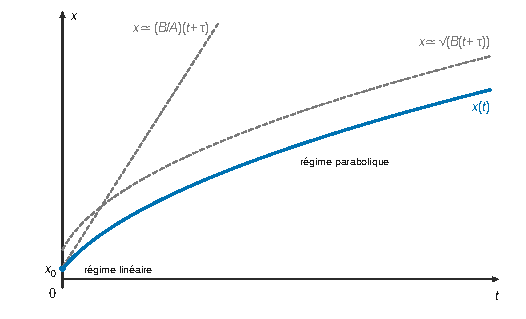
\includegraphics{figures/q44-croissance-oxyde.pdf}
\caption*{Figure 4 --- Épaisseur d'oxyde x(t) : régime linéaire puis régime
parabolique, la courbe restant sous ses deux asymptotes}
\end{figure}

\hypertarget{question-45}{%
\subsection{Question 45}\label{question-45}}

\begin{indication}{1}

Construisez un temps de diffusion sur l'épaisseur \(x\) et un temps d'épaississement \(x/\dot x\), puis formez leur rapport.

\end{indication}

\begin{indication}{2}

La quasi-stationnarité demande que le profil de concentration s'établisse bien plus vite que l'interface ne bouge. Le rapport obtenu ne fait intervenir que deux concentrations.

\end{indication}

\hypertarget{solution-44}{%
\subsubsection{Solution}\label{solution-44}}

Temps de diffusion à travers la couche : \(\tau_D\sim x^2/D\). Temps de croissance : \(\tau_c=x/\dot x=xN_v/J\), d'où

\equationajustee{\begin{aligned}
\tau_c&=\frac{xN_v}{C_g}\Big(\frac1{h_g}+\frac1{k_i}+\frac xD\Big)\\
&\geqslant\frac{N_v}{C_g}\cdot\frac{x^2}{D}
\end{aligned}}

d'où

\equationajustee{\boxed{\frac{\tau_c}{\tau_D}\geqslant\frac{N_v}{C_g}}}

L'égalité est atteinte dans le régime parabolique, le plus défavorable. La quasi-stationnarité exige \(\tau_D\ll\tau_c\), d'où la condition

\equationajustee{\boxed{C_g\ll N_v}}

Elle est largement vérifiée : pour un oxydant gazeux sous 1 bar vers 1000 °C, \(C_g=P/RT\approx9\ \mathrm{mol\cdot m^{-3}}\), alors que \(N_v\approx4\times10^4\ \mathrm{mol\cdot m^{-3}}\) (Q42). Il faut « vider » un grand volume de gaz pour former un petit volume d'oxyde condensé : la croissance est lente devant la diffusion.

\begin{piege}

Le temps de diffusion se compare au temps de déplacement de l'interface, pas à la durée totale de l'expérience : c'est le mouvement de l'interface qui rend le problème non stationnaire.

\end{piege}

\hypertarget{bilan}{%
\section{Bilan}\label{bilan}}

\textbf{Méthodes à retenir.}
- Loi exponentielle : un écart constant de l'argument donne un rapport constant (Q1, Q2). Pour une petite dérive, on différentie le logarithme (Q7, Q8).
- Compensation au premier ordre : on écrit la grandeur sous la forme \(1+(K_1-K_2)\theta\), on choisit les composants pour annuler la différence, puis on vérifie la dispersion des composants (Q8).
- ALI : on commence toujours par le régime de fonctionnement, qui se lit sur la topologie de la rétroaction (Q9, Q13). Oscillateur de relaxation : intégrateur et comparateur à hystérésis, avec des pentes et des seuils qui donnent la période (Q14 à Q18).
- Ailette : bilan sur une tranche, solution centrée sur l'extrémité, flux par la base, rendement \(\tanh(m\ell)/(m\ell)\). Tout dépend du nombre \(m\ell\) (Q21 à Q31).
- Thermochimie : critère quantitatif chiffré, chemin fictif pour la température de fin de réaction adiabatique, confrontation aux températures de fusion et d'inversion (Q33, Q34).
- Cinétique : relier la grandeur mesurée à l'avancement, linéariser la loi d'Arrhenius en \(\ln k\) contre \(1/T\) (Q35 à Q39).
- Transport en série : flux uniforme, résistances additives, régimes limités par l'étape la plus lente (Q43, Q44), quasi-stationnarité par comparaison de temps caractéristiques (Q45).

\textbf{Prérequis à revoir.} ALI idéal (régimes linéaire et saturé, suiveur, sommateur, comparateur à hystérésis), loi de Fourier et loi de Newton, fonctions hyperboliques, grandeurs standard de réaction (supposées indépendantes de \(T\)), loi d'Arrhenius, nombres d'oxydation.

\textbf{Questions classiques transposables.} L'ailette (Q21 à Q31) est un grand classique de la diffusion thermique. L'oscillateur à intégrateur et comparateur (Q13 à Q19) revient très souvent en électronique. Le modèle de Deal-Grove (Q43 à Q45) reproduit la structure de nombreux problèmes de corrosion ou d'oxydation sèche : flux en série, puis loi linéaire suivie d'une loi parabolique. Les ordres de grandeur sont à retenir :

\begin{itemize}
\tightlist
\item
  \(v=k_BT/q\approx25\ \mathrm{mV}\) ;
\item
  \(\ln2\ \mathrm{V^{-1}}\) pour un convertisseur à 1 V par octave ;
\item
  une vitesse de nitruration multipliée par environ 1,8 entre 1300 et 1400 °C pour \(E_a\approx130\ \mathrm{kJ\cdot mol^{-1}}\).
\end{itemize}

\end{document}
